\documentclass[11pt, a4paper]{article}

% ─── packages ────────────────────────────────────────────────────────────────
\usepackage[margin=2.5cm]{geometry}
\usepackage{amsmath, amssymb}
\usepackage{graphicx}
\usepackage{booktabs}
\usepackage{multirow}
\usepackage{hyperref}
\usepackage{xcolor}
\usepackage{caption}
\usepackage{subcaption}
\usepackage{float}
\usepackage{parskip}
\usepackage{microtype}
\usepackage{enumitem}
\usepackage{algorithm}
\usepackage{algpseudocode}

\hypersetup{colorlinks=true, linkcolor=blue!60!black, citecolor=blue!60!black, urlcolor=blue!60!black}

% ─── title ───────────────────────────────────────────────────────────────────
\title{%
  \textbf{Studying EvolBA on CIFAR-10:} \\[0.3em]
  \large Hyperparameter Tuning, Covariance Structure, \\
  and Corruption-Guided Subspace Search \\[0.2em]
  \normalsize Evolutionary Computing: Final Project Report
}
\author{Tommaso Tarantino}
\date{June 2026}

% ─────────────────────────────────────────────────────────────────────────────
\begin{document}
\maketitle
\tableofcontents
\newpage

% =============================================================================
\section{Abstract}
% =============================================================================

Adversarial examples expose a basic fragility of deep image classifiers: small, often imperceptible perturbations can flip a model's prediction. EvolBA~\cite{evolba2024} attacks this fragility under the hardest realistic threat model: hard-label black-box (HL-BB) access, where the attacker observes only the predicted class, by hybridising Sep-CMA-ES with the Boundary Attack. This project studies EvolBA's evolutionary core in a setting the original paper never tested: CIFAR-10's $32\times32$ resolution, against two WideResNet-28-10 targets (a standard model and an adversarially trained one), under a much smaller query budget. Low-resolution imagery is not simply a smaller, easier version of the same problem; it is the regime many real deployments actually operate in (compressed feeds, low-cost sensors, security cameras), and it disables the very fractal-based initialisation the original method relies on, since the frequency split that technique depends on collapses at this resolution. That makes CIFAR-10 a genuine stress test of EvolBA's evolutionary machinery, not an easier toy version of the original problem.

We first diagnose where the original recipe struggles in this new regime: its fractal-based initialisation degrades as expected at low resolution, a large share of the query budget is consumed by the directed step and its backtracking rather than genuine search, and, most importantly, the optimiser's progress plateaus almost immediately against the adversarially trained model. These diagnostics motivate two attempts at a fix, both kept entirely within the original pixel space: tuning the directed step-size scale alongside the other free hyperparameters through careful paired comparisons, and testing whether richer covariance structures can lift the optimiser past its plateau. Neither works well: hyperparameter tuning buys only modest gains, and no covariance structure beyond the simple diagonal helps, because pixel space is simply too high-dimensional for any within-algorithm fix to adapt within a realistic budget. This motivates our main contribution: rather than tuning the search algorithm further, we change the space it searches in. Building a low-dimensional subspace from a richer zoo of corruption directions than the handful used for initialisation (corruptions chosen because they cross the decision boundary with a small perturbation while staying visually close to the original image), together with a few frequency components, gives the search a head start over treating every pixel direction as equally relevant. Searching in this subspace substantially raises the ceiling that pixel-space search could not lift, and is, by construction, a good match for the simplifying assumptions that make Sep-CMA-ES efficient; the underlying plateau is reduced rather than eliminated, since Phase 3 still tapers off before the query budget is spent, just from a far better starting level. The resulting attack is markedly more sample-efficient and substantially more effective against the adversarially trained model, where pixel-space search had previously made almost no progress at all.

Overall, the project shows that EvolBA's headline mechanisms transfer to a much smaller, harder-budgeted setting only with care, and that the largest gains come not from tuning the evolutionary strategy itself, but from reshaping the search space it operates in using cheap, problem-specific structure discovered during diagnosis.

% =============================================================================
\section{The EvolBA Algorithm (Tajima \& Ono, 2024)}
\label{sec:evolba_paper}
% =============================================================================

An attacker does not need to see inside a classifier to break it: a perturbation found by trial and error, invisible to a human eye, can still flip the predicted label. The hardest realistic version of this threat is \textbf{hard-label black-box} (HL-BB) access: the attacker may query the model but observes only the predicted class, with no gradients, logits, or confidence scores; this is the setting faced by most commercial and proprietary APIs. Tajima and Ono~\cite{evolba2024} proposed \textbf{EvolBA} for exactly this setting: an evolutionary-strategy-based attack that keeps a Sep-CMA-ES search anchored to the decision boundary using ideas borrowed from the Boundary Attack~\cite{ba2017}.

\subsection{Overview}

EvolBA is a loop that takes an image already misclassified and progressively shrinks its perturbation relative to the original, while never letting it drift back across the decision boundary. We describe it here using the same three-phase breakdown used throughout this report (\S\ref{sec:decomposition}), so that the algorithm and our later instrumentation of it share one vocabulary:

\begin{enumerate}
  \item \textbf{Phase 1 (Initialisation): obtain a first adversarial example.} The search needs a concrete adversarial point to improve on. EvolBA manufactures one by blending fractal texture into the original image: the result, $m^{(0)}$, already crosses the decision boundary but is still structurally close to $x_{\mathrm{orig}}$.

  \item \textbf{Phase 2 (Boundary refinement): pull the starting point onto the boundary.} A binary search between $m^{(0)}$ and $x_{\mathrm{orig}}$ trades off ``closer to the original'' against ``still adversarial,'' giving the evolutionary loop a starting point already near the decision boundary rather than deep inside the misclassified region.

  \item \textbf{Phase 3 (ES optimisation): shrink the perturbation while staying adversarial.} This is the heart of the algorithm, repeated generation after generation: Sep-CMA-ES (diagonal covariance only, the only tractable choice at $n=3072$ or larger) samples a population of candidate perturbations around the current point $m^{(t)}$, the population's adversarial/non-adversarial split is used to shift the mean and set the next step size, and a short binary search then pulls the result back toward $x_{\mathrm{orig}}$, exactly as in Phase 2 but now every generation. Each generation thus simultaneously \emph{explores} (CMA-ES sampling) and \emph{exploits} (binary search toward $x_{\mathrm{orig}}$), so $m^{(t)}$ steadily contracts while staying just on the far side of the boundary; the exact mechanics are given below (\S\ref{sec:evolba_algorithm}). As an \emph{extra} mechanism within Phase 3, not a phase of its own, a periodic \textbf{jump operator} (every 1{,}000 queries) reinjects fractal texture into the current point if the search has stagnated, after which Phase 3 resumes as normal.
\end{enumerate}

\subsection{Objective Function}

EvolBA minimises the L2 norm of the perturbation subject to an explicit feasibility constraint:
\begin{align}
  \text{minimise} \quad & f(\tilde{x}) = \|\tilde{x} - x_{\mathrm{orig}}\| + f_p(\tilde{x}) \label{eq:obj} \\
  \text{subject to} \quad & \mathcal{C}(\tilde{x}) \neq \mathcal{C}(x_{\mathrm{orig}}) \label{eq:constraint}
\end{align}
where $f_p(\tilde{x}) = c_{\mathrm{pen}} = 1{,}000$ if non-adversarial and $0$ otherwise. The penalty is safely larger than any achievable L2 distance between two images with pixel values in $[0,1]$, guaranteeing that every adversarial candidate ranks above every non-adversarial one, while leaving the ranking within each side governed purely by L2 distance.

\subsection{Algorithm}
\label{sec:evolba_algorithm}

The EvolBA main loop repeats four processes per generation:

\begin{enumerate}[noitemsep]
  \item \textbf{Sample and evaluate offspring}: draw $\lambda$ candidates from $\mathcal{N}(m^{(t)}, \sigma^{(t)2} C^{(t)})$.
  \item \textbf{Update the mean direction}: compute weighted search direction $v^{(t)}$ using all $\lambda$ offspring, then $m^{(t+1)} \leftarrow m^{(t)} + \xi^{(t)} v^{(t)}$.
  \item \textbf{Adapt the step size}: compute $\xi^{(t)} = \|m^{(t)} - x_{\mathrm{orig}}\| / \sqrt{t}$, halve if the updated mean would leave the adversarial region (up to $\tau$ backtracks).
  \item \textbf{Move toward the original image}: binary search between $m^{(t+1)}$ and $x_{\mathrm{orig}}$.
\end{enumerate}

A critical difference from standard Sep-CMA-ES is the mean update: EvolBA uses \emph{all} $\lambda$ offspring, exploiting non-adversarial candidates by negating their direction:
\begin{equation}
  v^{(t)} = \frac{\displaystyle\sum_{i=1}^{l} w_i z_{i:\mu}^{(t)} - \sum_{j=l+1}^{\mu} w_j z_{(\mu-j+1):\mu}^{(t)}}{\left\| \displaystyle\sum_{i=1}^{l} w_i z_{i:\mu}^{(t)} - \sum_{j=l+1}^{\mu} w_j z_{(\mu-j+1):\mu}^{(t)} \right\|}
  \label{eq:meanshift}
\end{equation}

Another critical difference is the step size. EvolBA replaces CSA (Cumulative Step-size Adaptation) with a deterministic geometry-informed schedule:
\begin{equation}
  \xi^{(t)} = \frac{\|m^{(t)} - x_{\mathrm{orig}}\|}{\sqrt{t}}
  \label{eq:stepsize}
\end{equation}
CSA infers whether to grow or shrink $\sigma$ from the length of an accumulated evolution path of successive mean shifts: if consecutive steps keep pointing the same way, the path grows long and $\sigma$ increases; if they cancel out, the path stays short and $\sigma$ shrinks. This implicitly assumes the mean is converging toward a \emph{stationary} optimum, so that genuine progress shows up as correlated successive steps. That assumption does not hold here: process~4 of the loop continually pulls the mean back \emph{onto} the decision boundary via binary search, so $m^{(t)}$ oscillates near a moving target (the boundary itself shifts as the perturbation shrinks) rather than progressing smoothly toward a fixed point. CSA would read this healthy oscillation as anti-correlated steps, i.e.\ no progress, and respond by driving $\sigma$ toward collapse regardless of whether the search is actually working. The deterministic schedule in Eq.~\ref{eq:stepsize} sidesteps the problem entirely: it needs no feedback signal to interpret, and simply scales with the current distance from the original image.

On ImageNet, Tajima and Ono tuned EvolBA via preliminary experiments on VGG19 (50 images, up to 30,000 queries: $\sigma=10^{-3}$, $c_\mu=10^{-1}$, $\lambda=117$, jump timing at 1,000 queries) and reported it matching or beating HSJA and clearly beating the original Boundary Attack across four architectures (VGG19, ResNet-50, Inception-v3, ViT) at both 10k and 30k queries.

% =============================================================================
\section{Our Implementation: Adapting EvolBA to CIFAR-10}
\label{sec:our_impl}
% =============================================================================

Rather than simply reproducing EvolBA, we treat it first and foremost as an evolutionary-computing object of study: the central question throughout is how Sep-CMA-ES's search-distribution updates behave in this new, much smaller and much more tightly query-budgeted setting, and how they can be improved. The investigation is organised into two parts, each motivated by what came before:

\begin{description}[noitemsep]
  \item[Part 1 (Diagnosis and the limits of pixel-space fixes, \S\ref{sec:diagnosis}):] instrument the baseline end-to-end to find out, concretely, what breaks and why, then test two natural fixes, hyperparameter tuning and richer covariance structure, entirely within the original $n=3072$ pixel space.
  \item[Part 2 (Inductive bias in the search space, \S\ref{sec:inductive_bias}):] once Part 1 shows that neither fix lifts the plateau by much, redesign the search space itself using the corruption directions surfaced during diagnosis.
\end{description}

Throughout, ``Phase 1/2/3'' refers to EvolBA's own three-step attack loop (initialisation, boundary refinement, ES optimisation, defined in \S\ref{sec:decomposition}), while ``Part 1--2'' refers to the two stages of this project's investigation. Across both parts, comparisons are \emph{paired}: the same image, model, and random seed are used under every condition being compared.

\subsection{Setting}

We study EvolBA in a setting that differs from the original paper in three deliberate ways:

\textbf{(1) CIFAR-10 instead of ImageNet.} We use $32\times32$ RGB images ($N = 3072$) rather than ImageNet's $224\times224$ ($N = 150{,}528$). This is not simply a smaller, easier version of the same problem: low-resolution imagery is itself the regime many real deployments operate in (compressed video feeds, low-cost sensors, security cameras), and, more importantly for this study, it is a genuinely harder setting for EvolBA specifically. At only 32 frequency bins per axis, the DFT-based low/high-frequency split that EvolBA's fractal initialisation relies on collapses: ``structure'' and ``texture'' are squeezed into a much narrower band, blurring the very distinction the fractal technique exploits. This single resolution change disables a core mechanism of the original method, which is one motivation for exploring a corruption-family Phase 1 instead. For the same reason, we do not carry the paper's \textbf{jump operator} (\S\ref{sec:evolba_paper}) into our final implementation: it escapes stagnation by re-blending fractal texture into the current point, the identical DFT-based trick whose low/high-frequency split degrades at $32\times32$, so it would inherit the same weakness mid-search that motivates dropping it from initialisation. Stagnation, the failure mode the jump operator is meant to rescue, is diagnosed directly in Part 1 (\S\ref{sec:diagnosis}), where we also test whether richer covariance structure can address it, and is substantially though not completely reduced in Part 2. The smaller image size also has a practical upside, making it tractable to attack hundreds of images across many configurations on commodity hardware, but the resolution drop is best read as trading one difficulty (scale) for another (no usable fractal initialisation), not as a simplification.

\textbf{(2) Standard and robust WideResNet-28-10.} WRN-28-10 is the de facto reference architecture for CIFAR-10 robustness research, the backbone behind most top-ranked entries on RobustBench (\url{https://robustbench.github.io}). Using a single architecture in two training configurations, (a) \emph{standard} CE training ($\sim$93\% clean accuracy) and (b) \emph{robust} TRADES training (Wang et al.~\cite{wang2023}, $\sim$92.4\% clean, $\sim$67.3\% robust under L$_\infty$ $\varepsilon=8/255$), isolates the effect of the training procedure on attack difficulty while keeping architecture effects constant.

\textbf{(3) Budget of hundreds to a few thousand queries.} The original paper allows up to $30{,}000$ queries. CIFAR-10's $50\times$ smaller search space should require correspondingly fewer samples to explore, so we test whether comparable attack quality is reachable in a small fraction of the queries the original paper needed.

\subsection{Decomposition into Analysis Phases}
\label{sec:decomposition}

We decompose the EvolBA loop into three separable components:

\begin{description}[noitemsep]
  \item[Phase 1 (Initialisation):] find any adversarial example (starting point).
  \item[Phase 2 (Boundary refinement):] binary search between $x_{\mathrm{orig}}$ and the Phase 1 output to reach a point close to the decision boundary.
  \item[Phase 3 (ES optimisation):] run the Sep-CMA-ES loop to minimise L2 while remaining adversarial.
\end{description}

The improvement ratio
\[
  \mathrm{IR} = \frac{\text{init\_l2} - \text{best\_l2}}{\text{init\_l2}}
\]
is our headline metric throughout, where \texttt{best\_l2} is the running minimum of $\|m^{(t)}-x_{\mathrm{orig}}\|$ over the whole trajectory. We also define $\mathrm{IR}_\text{phase3} = (\text{phase1\_l2}-\text{best\_l2})/\text{phase1\_l2}$ and $\mathrm{IR}_\text{total}$ which accounts for the Phase 1 starting position relative to uniform-random initialisation.

\textbf{Image sample.} Most experiments default to 200 CIFAR-10 images jointly correctly classified by both models (20 per class), paired across conditions with matching seeds; individual studies note where they use a smaller diagnostic sample or a larger validation one.

% =============================================================================
\section{Part 1: Diagnosis and the Limits of Pixel-Space Fixes}
\label{sec:diagnosis}
% =============================================================================

Before tuning anything, we instrumented our finetuned EvolBA baseline (already adapted per \S\ref{sec:our_impl}, with the jump operator dropped) end-to-end on CIFAR-10 to find out, concretely, what works, what breaks, and why. Diagnosis surfaces two actionable symptoms: a directed-step/backtracking mechanism that dominates query cost, and a search procedure that stagnates almost immediately against the robust model. We then try to fix these in two different ways, entirely within the original pixel space: by tuning hyperparameters, and by giving Sep-CMA-ES a richer covariance structure. As this section shows, neither fix moves the needle by much. (A third diagnostic finding, that the paper's fractal initialisation can be replaced by a cheaper, equally effective family of image corruptions, matters most for Part 2, so it is described there instead, \S\ref{sec:inductive_bias}, where it is actually put to use.)

\subsection{Query Cost Breakdown}

To find out where the query budget is actually spent, we instrumented the baseline end-to-end (8 images $\times$ 2 models, paper hyperparameters, $\lambda=28$, budget 3{,}000 queries) and logged a per-generation breakdown of every query.

\begin{table}[htbp]
\centering
\caption{Per-generation query-cost breakdown under baseline hyperparameters, 8 images $\times$ 2 models.}
\label{tab:diag_query}
\begin{tabular}{lcc}
\toprule
 & Standard & Robust \\
\midrule
Offspring evaluation (q/gen) & $\approx28$ & $\approx28$ \\
$\xi$-shrink loop (q/gen)    & $\mathbf{63.6}$ & $\mathbf{143.2}$ \\
Backtracking (q/gen)         & $0.57$ & $1.93$ \\
\textbf{Total (q/gen)}       & $\approx92$ & $\approx173$ \\
Mean generations completed (3{,}000-query budget) & $\approx23$ & $\approx12$ \\
\bottomrule
\end{tabular}
\end{table}

The $\xi$-shrink loop and backtracking together account for roughly \textbf{75\% of every query spent}, on both models: the directed mean-shift step, not offspring evaluation, dominates the cost of each generation. Tracking the running-best L2 across the run, the standard model shows a sharp breakthrough around generation 12--13 followed by a plateau ($\approx65\%$ total improvement), while the robust model stays close to flat throughout ($\approx4\%$ total improvement): cost-effectiveness (L2 improvement per query) falls steadily as a run progresses, with the back third of any run buying measurably less than the first two-thirds.

\begin{figure}[htbp]
\centering
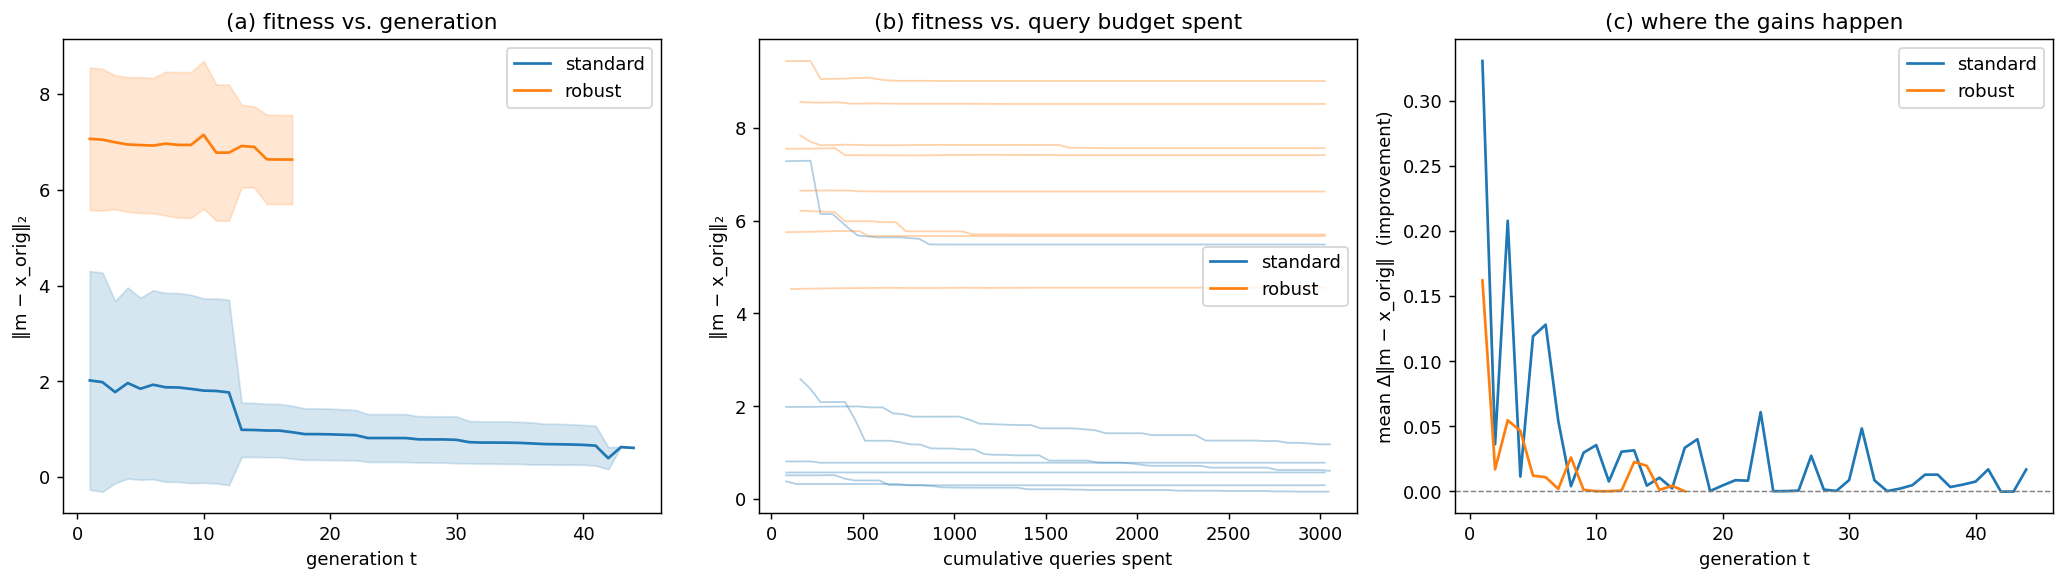
\includegraphics[width=\textwidth]{figures/study1_fitness_curves.png}
\caption{L2-to-original ($\|m^{(t)}-x_{\mathrm{orig}}\|_2$) over the course of a run, standard vs.\ robust model. (a) vs.\ generation: the standard model breaks through around generation 12--13 then flattens; the robust model stays nearly flat throughout. (b) the same curves vs.\ cumulative queries spent, showing the plateau in budget terms. (c) per-generation improvement: gains are front-loaded on both models, with the robust model's already-small gains vanishing almost completely after the first few generations.}
\label{fig:fitness_curves}
\end{figure}

Since the directed mean-shift step and the backtracking it sometimes triggers dominate the per-generation cost so heavily, the hyperparameters governing them (the step's scale, and the backtracking budget $\tau$) are natural candidates to tune, taken up directly next (\S\ref{sec:finetuning}).

\subsection{Failure Modes and the Phase 3 Plateau}

To separate Phase 1 (initialisation) quality from Phase 3 (search) quality, we ran a $2\times2$ design (100 images $\times$ 2 models $\times$ 2 initialisation methods, 400 attacks) and classified every run into one of four buckets by improvement ratio: \textit{hard} (Phase 1 itself failed), \textit{flat} (IR$<5\%$), \textit{partial} ($5$--$50\%$), \textit{good} (IR$\geq50\%$).

\begin{table}[htbp]
\centering
\caption{Failure-mode taxonomy, 100 images $\times$ 2 models $\times$ 2 initialisation methods.}
\label{tab:diag_failure}
\begin{tabular}{lccccc}
\toprule
Condition & hard & flat & partial & good & mean IR \\
\midrule
standard / uniform & 0\% & 11\% & 59\% & 30\% & 0.386 \\
standard / fractal & 0\% & 22\% & 64\% & 14\% & 0.274 \\
robust / uniform   & 10\% & 47\% & 42\% & 1\% & 0.088 \\
robust / fractal   & 3\% & 49\% & 47\% & 1\% & 0.090 \\
\bottomrule
\end{tabular}
\end{table}

Two findings stand out. First, \textbf{Phase 3 is the dominant bottleneck for the robust model regardless of initialisation}: mean IR sits at $\approx0.09$ whether Phase 1 uses uniform-random or fractal seeding, and $96\%$ of robust-model runs land in \textit{flat} or \textit{partial}, meaning the search itself stagnates almost immediately rather than failing to start. Second, \textbf{initial L2 does not predict Phase 3 success}: the correlation between starting distance and improvement ratio is weak or near zero in three of four conditions (Pearson $r\in[-0.02, 0.45]$), so simply moving the starting point closer to the original image, without changing how Phase 3 searches, cannot by itself rescue the robust attack.

This stagnation is the central open problem left by diagnosis: the search makes most of its progress in the first few generations and then plateaus, especially against the robust model. Hyperparameter tuning (\S\ref{sec:finetuning}) can shift the height of this plateau, but as the covariance-structure attempt below (\S\ref{sec:cma_alt}) confirms, no choice of covariance representation in pixel space removes it. This motivates the search-space change introduced in Part 2 (\S\ref{sec:inductive_bias}), which reduces the plateau substantially but, as we will see, does not eliminate it either.

\subsection{Attempt 1: Hyperparameter Tuning}
\label{sec:finetuning}

The query-cost finding above motivates tuning the directed step-size scale $\xi_{\text{step\_scale}}$ (a free multiplier on Eq.~\ref{eq:stepsize}), the binary-search budget, the backtracking budget $\tau$, and population size $\lambda$. We implemented EvolBA's Sep-CMA-ES loop faithfully in the full $n=3072$ pixel space (verified term-by-term against the paper's equations and algorithms) and swept each hyperparameter through paired comparisons (same image and seed across conditions), then tested whether the individually-best choices compound when combined.

Two results matter most. First, $\xi_{\text{step\_scale}}$ is far more sensitive than the other knobs: sweeping it from $0.018$ to $2.0$ shows the paper's own value ($1.0$) is close to optimal on the standard model ($\mathrm{IR}=0.406$), while $0.5$ is best on the robust model ($\mathrm{IR}=0.066$) and $2.0$ overshoots catastrophically \emph{on the robust model specifically} ($\mathrm{IR}=-0.058$, worse than the starting point, even though the standard model is still fine at that scale). No single value wins on both models, so any choice is a compromise rather than a fix. (The backtracking budget $\tau$ was swept too, but with no clear winner: $\tau=0$ reaches a slightly better median final L2, but with higher variance and a tradeoff early in a run, so we read this as inconclusive rather than as a basis for a default choice; a free efficiency gain, detecting float32 binary-search saturation early, survives regardless and is adopted throughout.) Second, and most importantly, \textbf{these individually-validated choices do not compound}: combining $\xi_{\text{step\_scale}}=0.5$, $\tau=0$, and adaptive binary search into one configuration and testing it at the paper's own $\lambda=28$ is a wash on the standard model and a loss on the robust one ($\mathrm{IR}=0.380$/$0.047$ vs.\ baseline's $0.386$/$0.060$). The reason is that $\lambda$ is not an independent knob: it determines which step-size regime is optimal, so a recipe validated at one $\lambda$ does not transfer cleanly to another.

\begin{table}[htbp]
\centering
\caption{Pixel-space hyperparameter tuning: paper baseline vs.\ best validated configuration, $Q=2000$.}
\label{tab:tuning_summary}
\begin{tabular}{lcc}
\toprule
Configuration & Standard IR & Robust IR \\
\midrule
Paper baseline ($\xi_{\text{step\_scale}}=1.0$, $\tau=3$, $\lambda=28$, fixed BS) & 0.386 & 0.057 \\
\textbf{Best validated} ($\xi_{\text{step\_scale}}=0.5$, $\tau=0$, $\lambda=14$, adaptive BS) & \textbf{0.441} & \textbf{0.071} \\
\bottomrule
\end{tabular}
\end{table}

The improvement is small: an absolute IR gain of only $+0.055$ on the standard model and $+0.014$ on the robust model, and it does not even survive a switch back to the paper's own $\lambda=28$. This is the single best combination found in the sweep, not a strongly validated recommendation; given the chapter's overall message, we would not read much into it being reproduced exactly. The honest reading is that the paper's original hyperparameters were already close to a local optimum for pixel-space Sep-CMA-ES, and that remains true even after porting the algorithm to a much smaller, lower-resolution, far more tightly query-budgeted regime than the one it was designed for.

Figures~\ref{fig:pixel_grid_standard} and~\ref{fig:pixel_grid_robust} show this best validated configuration running on the same five images used later for Part 2's validation figures (\S\ref{sec:final_run}), tracked through the same checkpoint scheme, for a direct visual comparison. On the standard model, the perturbation is visibly noisy and speckled rather than structured, and still manages a real reduction in L2 over the run. On the robust model, one of the five images fails Phase 1 entirely (uniform-random initialisation never finds an adversarial point within the attempt budget, the same ``hard'' failure mode quantified in \S\ref{sec:diagnosis}), and for the remaining four, L2 barely moves at all across the whole of Phase 3: the plateau diagnosed earlier in this part is plainly visible, not just a property of the summary statistics.

\begin{figure}[htbp]
\centering
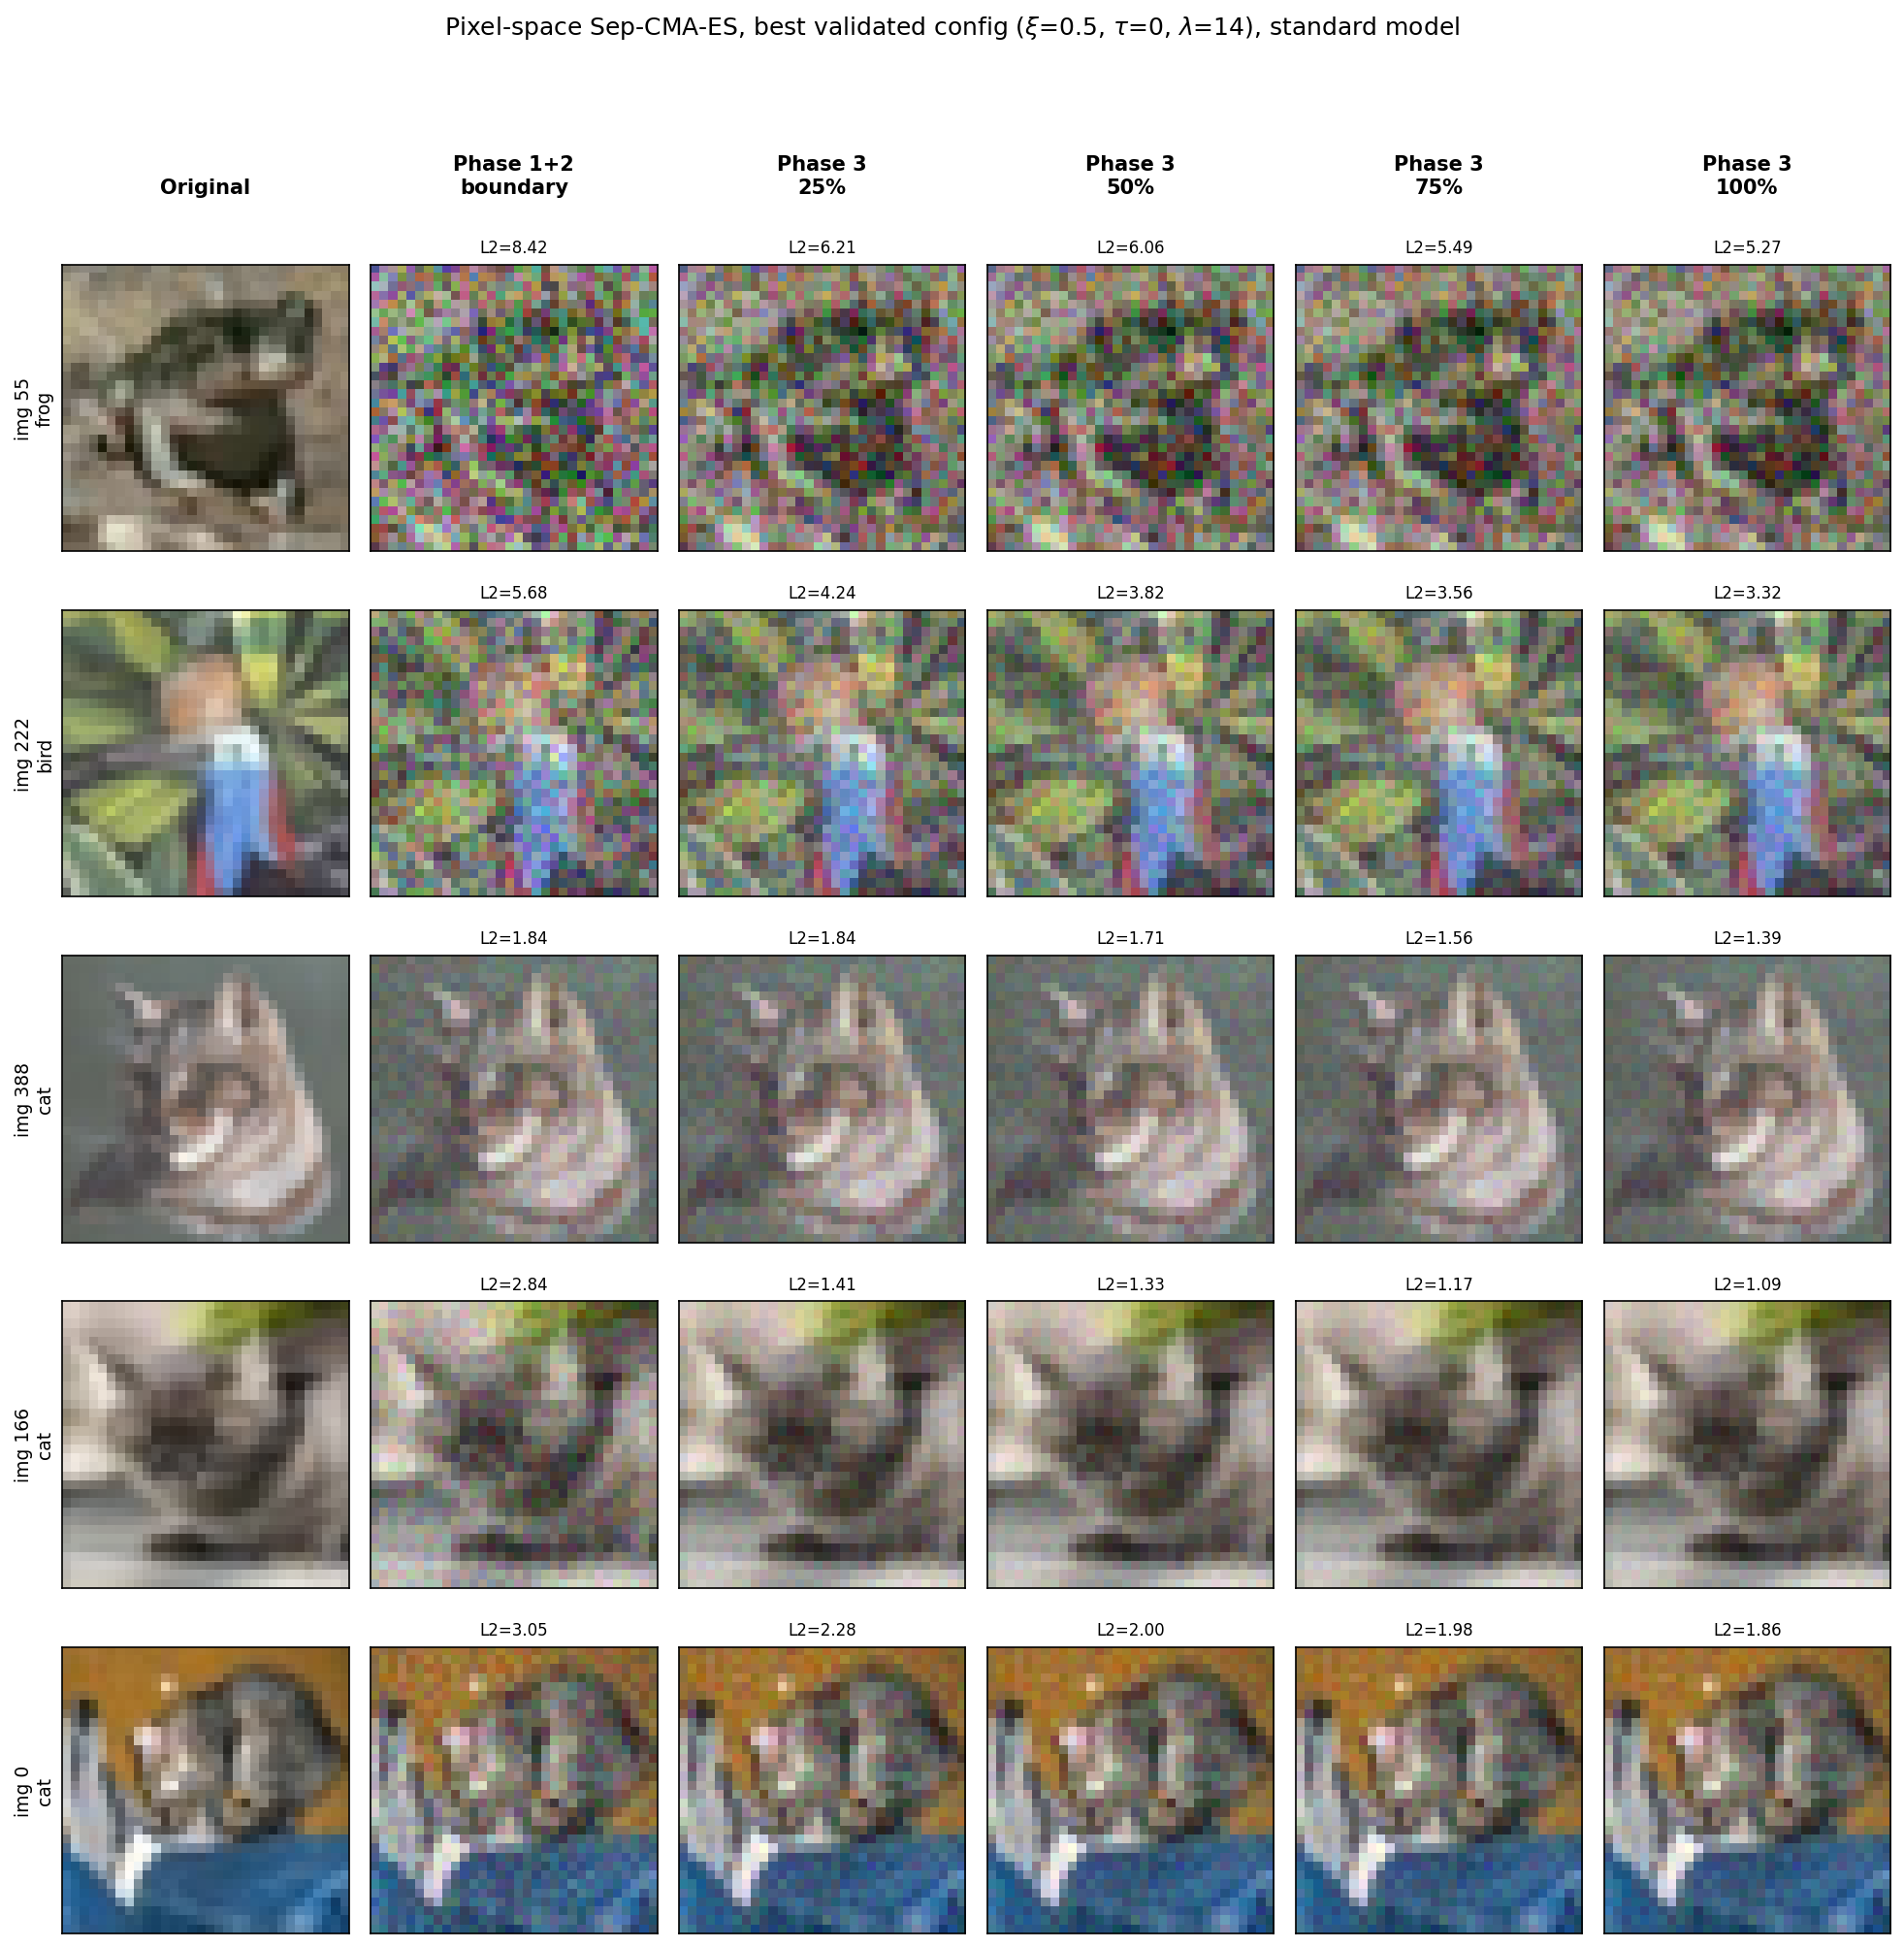
\includegraphics[width=\textwidth]{figures/pixel_space_snapshot_grid_standard.png}
\caption{Pixel-space Sep-CMA-ES at the best validated configuration, standard model, same five images and checkpoint scheme as Figures~\ref{fig:final_grid_standard}/\ref{fig:final_grid_robust}. The perturbation is visibly noisy rather than structured, in contrast to the corruption-subspace result in Part 2.}
\label{fig:pixel_grid_standard}
\end{figure}

\begin{figure}[htbp]
\centering
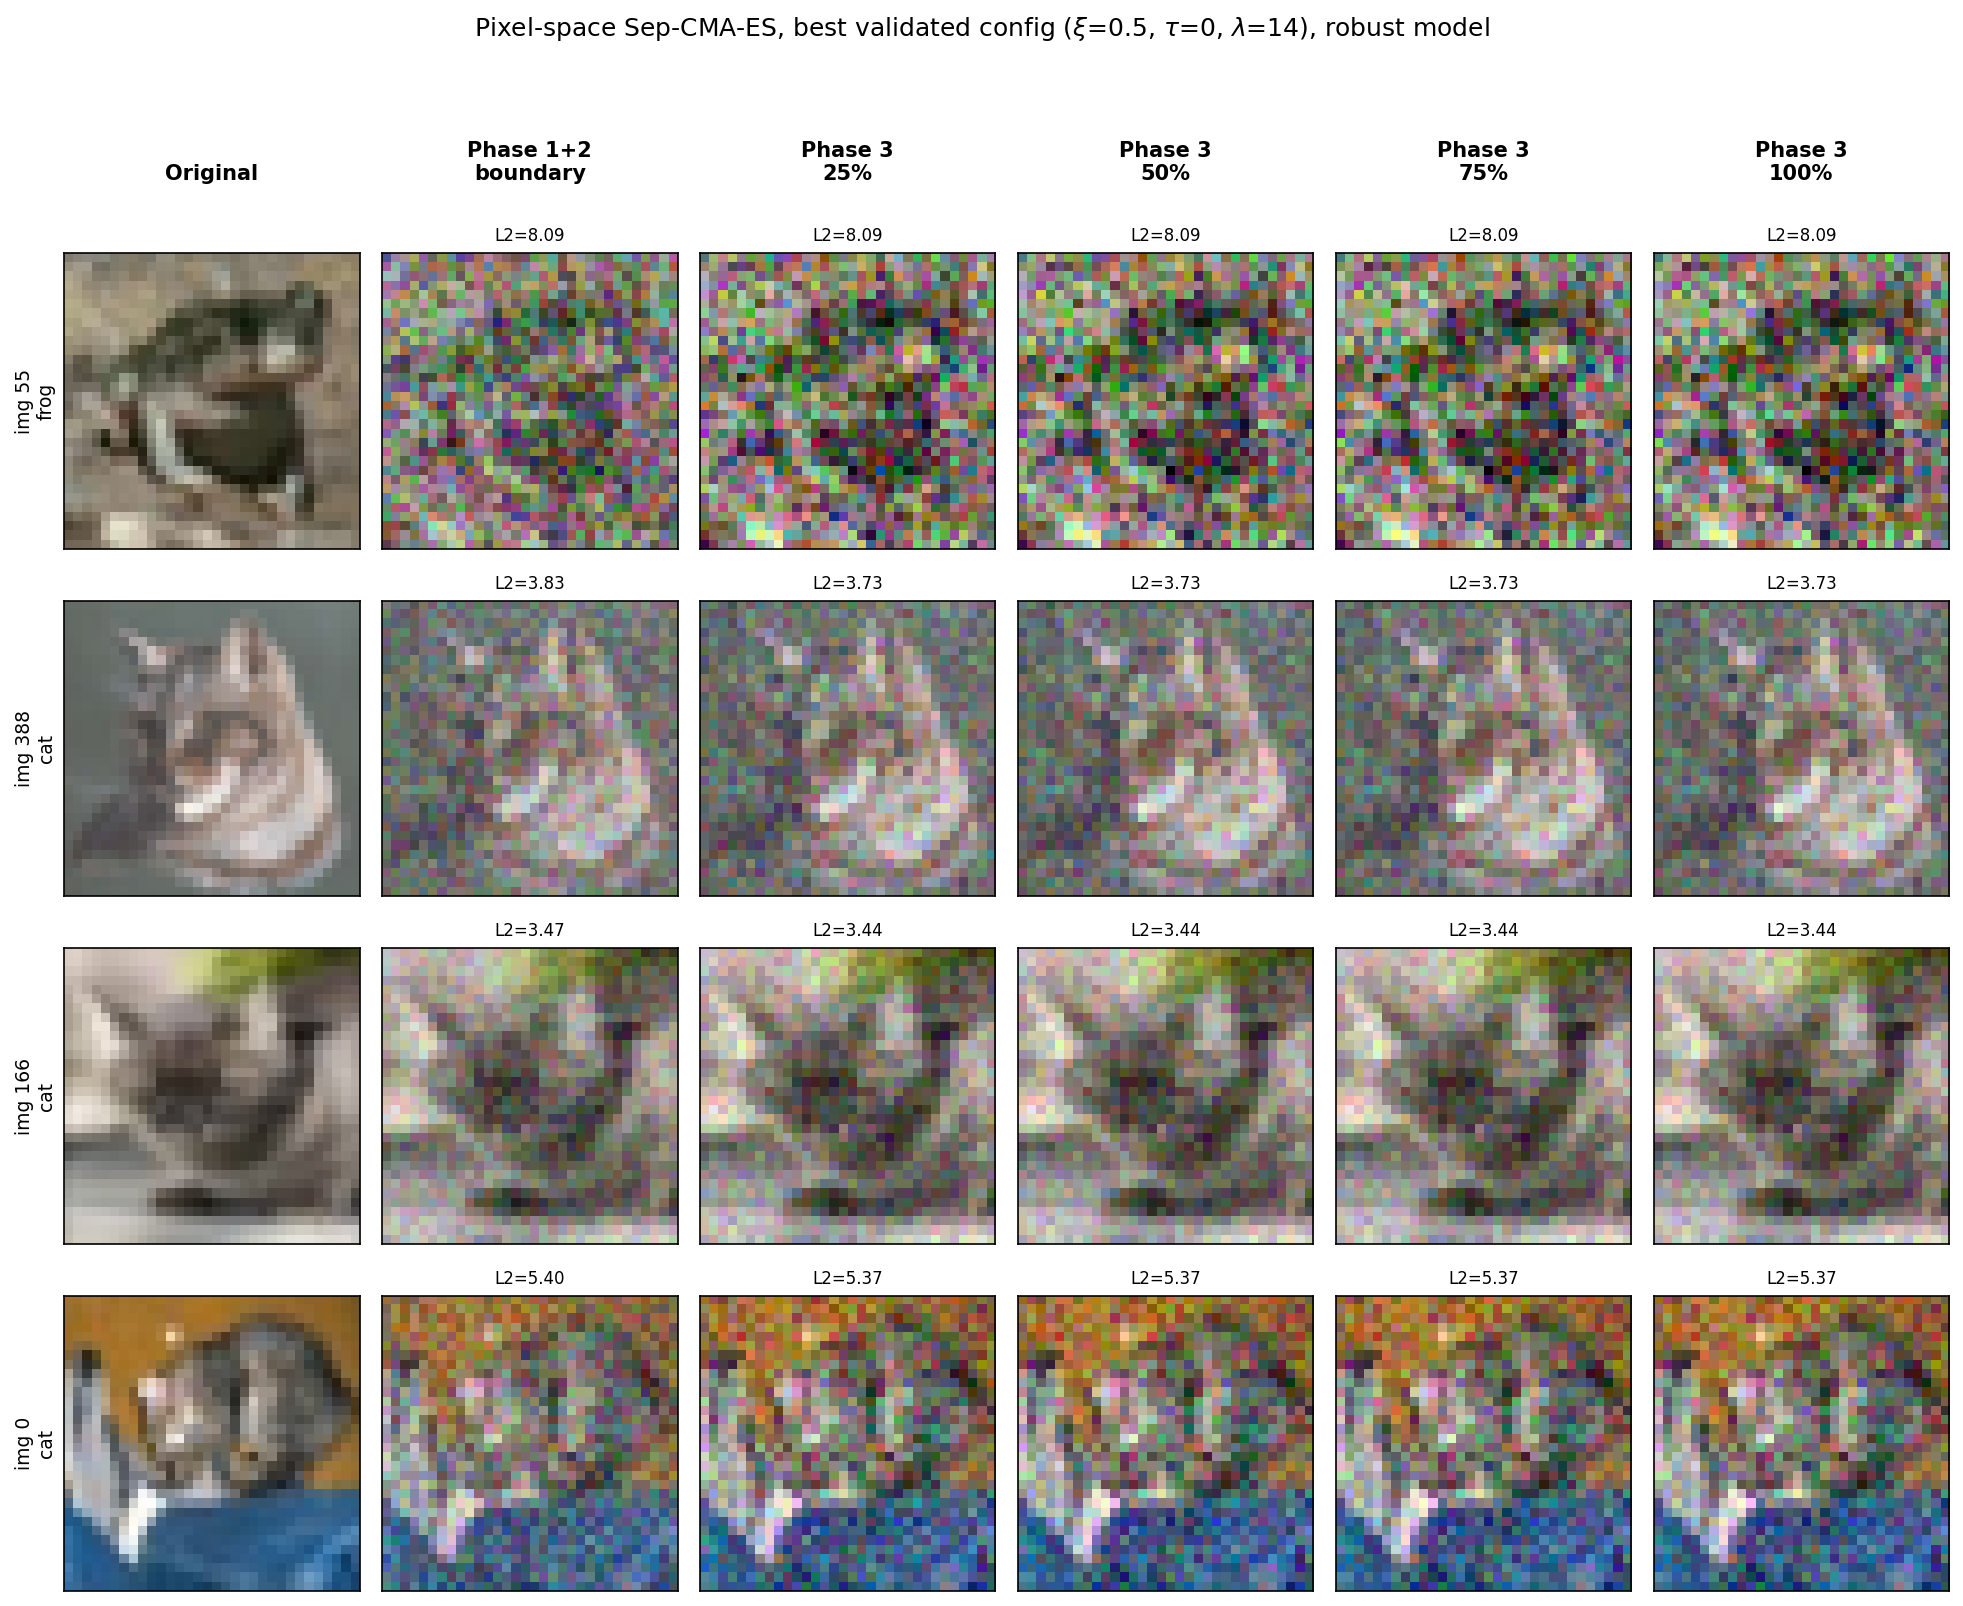
\includegraphics[width=\textwidth]{figures/pixel_space_snapshot_grid_robust.png}
\caption{Same configuration and checkpoints, robust model. One image (a Phase 1 failure) is omitted. L2 is nearly frozen across all of Phase 3 for every remaining image, a direct visual counterpart to the near-zero robust-model IR reported in Table~\ref{tab:tuning_summary}.}
\label{fig:pixel_grid_robust}
\end{figure}

\subsection{Attempt 2: Richer Covariance Structure}
\label{sec:cma_alt}

Sep-CMA-ES uses only a \emph{diagonal} covariance. This attempt asks whether covariance structure \emph{beyond} the diagonal can lift the optimiser past the plateau just diagnosed, in this short-horizon (10--60 generation), pixel-space regime. We compared five conditions sharing one fixed carrier ($\xi_{\text{step\_scale}}=0.5$, Attempt 1's step-size finding, together with adaptive binary search, but otherwise the paper's own $\lambda=28$ and $\tau=3$, not Attempt 1's single best combination), differing only in covariance representation: plain \texttt{sep} ($k{=}0$); VkD-CMA, $C=D(I+VV^\top)D$ with $V\in\mathbb{R}^{n\times k}$ a rank-$k$ correction to the diagonal ($k\in\{1,2,3\}$); and $(1{+}1)$-CMA-ES (\texttt{o11}), elitist, one query per generation, $p_{\text{succ}}$-based step adaptation. Using one fixed carrier for all five conditions biases the comparison somewhat in favour of \texttt{sep}, since $\lambda=28,\tau=3$ is closer to what \texttt{sep} was already shown to tolerate well; a separate tuning pass per variant was not feasible within this project's budget, but Attempt 1 already showed the tuning gain over untuned defaults is small, so this bias is unlikely to change the conclusion below.

A full, dense covariance was not tested directly: at $n=3072$ it would cost $O(\mu n^2)\approx2.6\times10^8$ operations per generation update and $O(n^3)\approx2.9\times10^{10}$ for eigendecomposition (vs.\ $O(n)\approx3$K for diagonal), and more importantly it has $9.4$M free parameters to learn; no population size that fits within our query budget could meaningfully explore a space that large.

\begin{table}[htbp]
\centering
\caption{Covariance-structure comparison, $N=100$, $Q=2000$, $\lambda=28$, $\tau=3$.}
\label{tab:ec1}
\begin{tabular}{lcccccc}
\toprule
 & \multicolumn{3}{c}{Standard (median\_init $=3.99$)} & \multicolumn{3}{c}{Robust (median\_init $=7.50$)} \\
\cmidrule(lr){2-4}\cmidrule(lr){5-7}
Condition & Med.\ best L2 & IR & Med.\ gens & Med.\ best L2 & IR & Med.\ gens \\
\midrule
\textbf{sep ($k{=}0$)} & \textbf{2.702} & \textbf{0.319} & 30 & 6.908 & 0.044 & 10 \\
vd1 ($k{=}1$) & 2.799 & 0.311 & 30 & 6.917 & 0.045 & 11.5 \\
vd2 ($k{=}2$) & 2.792 & 0.298 & 29 & 6.912 & 0.049 & 11.5 \\
vd3 ($k{=}3$) & 2.745 & 0.298 & 30 & \textbf{6.902} & \textbf{0.044} & 11 \\
o11            & 2.901 & 0.267 & 478 & 6.941 & 0.053 & 473.5 \\
\bottomrule
\end{tabular}
\end{table}

None of the five conditions beat plain \texttt{sep}-CMA-ES. The VkD variants are statistically indistinguishable from it (win rates $40$--$44\%$, median relative difference only $0.0$--$0.3\%$) no matter how much rank-$k$ correction is added. \texttt{o11} loses clearly on the standard model (median relative dis-improvement $-6.6\%$) despite running $\sim$16$\times$ more generations (478 vs.\ 30), and on the robust model only nudges ahead on the easier images while losing by more on the harder ones, leaving its median best-L2 ($6.941$) still slightly worse than \texttt{sep}'s ($6.908$). The one informative result is \texttt{o11}'s underperformance: discarding the population for a single elitist candidate consistently hurts, even with far more generations to compensate, which suggests EvolBA's evolutionary, population-sampling character is doing genuine work rather than just adding overhead.

This attempt therefore also fails to lift the plateau: the plateau is a function of pixel-space dimensionality itself, not of covariance representation.

\subsection{Summary: Why Pixel-Space Fixes Don't Work}

Tuning hyperparameters and enriching covariance structure each leave the plateau essentially where diagnosis found it: the best hyperparameter tuning available gains only $+0.055$/$+0.014$ IR over the paper's defaults, and none of four covariance variants beyond the diagonal beat the simple baseline. Both attempts are bounded by the same wall: $n=3072$ pixel directions is too large and unstructured a space for any amount of within-algorithm tuning to fix. The overwhelming majority of these directions are either insensitive to the decision boundary or destroy the image's structure before they help, and with only $\lambda\approx14$--$28$ samples per generation there is no way to tell in advance which few directions belong to the useful minority. The problem is structural, not parametric, and is addressed directly in Part 2 by changing the search space itself rather than the algorithm searching it.

% =============================================================================
\section{Part 2: Introducing Inductive Bias in the Search Space}
\label{sec:inductive_bias}
% =============================================================================

Neither attempt in Part 1 lifted the plateau by much, because neither changed the one thing that actually bounds it: the size and structure of the space being searched. This part addresses that directly by replacing the $n=3072$ pixel-direction space with a small, hand-built subspace of corruption directions, chosen because they are coherent, global image transformations the model is more likely to respond to, rather than arbitrary per-pixel noise. This part asks whether such a structured low-dimensional subspace can substantially raise the ceiling Part 1 could not; as the results below show, it does, though it does not make the underlying plateau disappear entirely.

\subsection{Corruption Family Selection}
\label{sec:corruption_family}

The paper's fractal initialisation generates an AE by blending fractal high-frequency content into the original image; \S\ref{sec:our_impl} already noted that this technique degrades at $32\times32$ resolution. Before building a search space out of corruption directions, we first ask a narrower question: can structured image corruptions, without any fractal image library, provide an equivalent or better source of adversarial directions to begin with? The underlying goal is to find corruptions that cross the decision boundary while leaving the image's structure essentially intact to a human observer, not merely ones that cross the boundary cheaply in pixel space.

\textbf{Why SSIM, not L2.} What we actually want to minimise is human-perceived change, which has no closed-form expression and must be approximated. L2 is the metric used everywhere else in this report, and it is a good choice for guiding the search later on: it is cheap, and as a proper norm it behaves predictably under interpolation, which is exactly what an optimiser that takes small steps and reasons about distances needs. But L2 is a poor proxy for what a human would actually notice, because it has no notion of \emph{where} a change falls: it is just a sum of squared per-pixel differences, blind to whether those pixels form a meaningful edge or texture or sit in a flat, unimportant region. A corruption can therefore reach the boundary with a small L2 budget while still visibly destroying the image's structure, simply because L2 cannot distinguish a change that respects that structure from one that does not. SSIM instead compares local structure directly, which tracks human perception of similarity considerably better. For that reason we use SSIM, not L2, to choose between corruptions in this section.

\textbf{Methodology.} Because Phase 1's query cost is sensitive to which corruption is tried, the choice of which few corruptions to use there deserves real scrutiny: we evaluated 9 candidate corruption types on 200 CIFAR-10 images correctly classified by both models, combining L2, SSIM, and visual inspection rather than relying on any single metric. For each (image, corruption, model) triple, a 12-step binary search on severity $s \in [0,1]$ finds the minimum severity that flips the prediction, and we record SSIM at that boundary point.

\textbf{Results.}

\begin{table}[htbp]
\centering
\caption{Mean SSIM at the decision boundary, 200 images, both WRN-28-10 models. Higher = better.}
\label{tab:stage0}
\begin{tabular}{lccc}
\toprule
Corruption & Standard SSIM & Robust SSIM & Category \\
\midrule
\texttt{jpeg\_compression} & 0.93 & 0.86 & Frequency domain \\
\texttt{brightness\_shift} & 0.91 & 0.78 & Global luminance \\
\texttt{contrast\_shift}   & 0.82 & 0.80 & Global dynamic range \\
\texttt{cutout}            & 0.87 & 0.81 & Local masking \\
\texttt{low\_freq\_noise}  & 0.81 & 0.66 & Smooth additive \\
\texttt{motion\_blur}      & 0.79 & 0.73 & Directional spatial \\
\texttt{gaussian\_noise}   & 0.82 & 0.57 & Broadband additive \\
\texttt{rgb\_fractal}      & 0.58 & 0.64 & Structured texture \\
\texttt{pixelation}        & 0.65 & 0.43 & Spatial resolution \\
\bottomrule
\end{tabular}
\end{table}

\textbf{Selected corruption family.} Four corruption types are selected as the Phase 1 pool:

\begin{enumerate}[noitemsep]
  \item \textbf{JPEG compression}: highest SSIM on both models (0.93/0.86). Removes high-frequency texture via DCT block quantisation, the same texture CNNs rely on.
  \item \textbf{Brightness shift}: pure uniform luminance reduction. Zero structural distortion; high SSIM (0.91) despite a large raw pixel shift.
  \item \textbf{Contrast shift}: squeezes pixel values toward the channel mean. Complementary failure mode to brightness shifts.
  \item \textbf{Low-frequency noise}: spatially correlated smooth additive noise, a different perturbation direction from the other three.
\end{enumerate}

The four are structurally independent perturbation directions. \textbf{Per-image selection}: all four are applied and the one with the highest SSIM at the boundary is selected. A hybrid fallback (a Dirichlet-mixed combination of all four) handles images where no single corruption crosses the boundary within $s\in[0,1]$. Some of these directions, alongside several additional ones (Table~\ref{tab:direction_zoo} below), reappear as literal search-space basis vectors later in this part.

\textbf{Validation against uniform-random initialisation (Study 2).} A follow-up comparison of eight corruption-based initialisers (including the four above) against uniform-random noise confirms the family is worth using: the best-of-pool strategy per image reduces the starting L2 substantially, from $3.80$ to $2.21$ on the standard model ($-40\%$) and from $7.51$ to $4.97$ on the robust model ($-34\%$), with Gaussian blur alone the strongest single strategy (winning on $53\%$ of standard / $70.5\%$ of robust images). This is a Phase 1/2 effect only: it says nothing about whether a better starting point also helps Phase 3 search, which Q1 below (\S\ref{sec:q1_phase1}) takes up directly.

\subsection{Subspace Construction ($k=14$)}
\label{sec:subspace_construction}

\textbf{Mechanism.} For each of 11 corruption types, we compute a single direction vector $d_c = x_c - x_{\mathrm{orig}}$, then L2-normalise it. For 8 of the 11, $x_c$ is the output of a fixed, hardcoded corruption function (\texttt{DIRECTION\_ZOO}, Table~\ref{tab:direction_zoo}), evaluated once with zero oracle queries. Each of these 8 functions hardcodes its \emph{own} parameter: there is no shared ``severity'' scale across types, and no documented selection procedure behind these specific values; they are constants fixed in the implementation. This looser selection criterion is deliberate, not an oversight. Phase 1's corruption family (\S\ref{sec:corruption_family}) was screened carefully, because the wrong choice there directly inflates query cost, so only a few types worth using were kept. The subspace basis has the opposite risk profile: an extra candidate direction is just extra raw material, since Phase 3's CMA-ES can re-weight or ignore unhelpful ones (see ``How much does this actually justify?'' below), so \texttt{DIRECTION\_ZOO} trades careful screening for breadth, including several corruption types (inversion, hue shift, posterize, sharpen, saturation, gamma) that were never put through Phase 1's SSIM evaluation at all. For the remaining 3 (jpeg, blur, fractal\_random), $x_c$ is instead the actual per-image decision-boundary point found by binary search during Phase 1 (\S\ref{sec:diagnosis}), a real adversarial point for that specific image, not a hardcoded one. Three DCT-II frequency-band vectors are appended in the same way, giving up to 14 vectors total. \textbf{Crucially, all 14 vectors are computed once per image, before Phase 3 starts, and never touched again}: the corruption and DCT functions are not called inside the generation loop. Phase 3 only ever samples linear-combination coefficients $\theta\in\mathbb{R}^k$ over these frozen vectors, mapping back to pixel space via $\delta = \theta^\top B$ for the basis $B$ described next.

\begin{table}[htbp]
\centering
\caption{\texttt{DIRECTION\_ZOO}: all 11 corruption-direction functions, with the exact hardcoded constant used by each. For 8 of these (all but jpeg, blur, fractal\_random), this fixed-parameter version is exactly what Phase 3 uses; for the other 3, it is superseded by the real per-image boundary point found during Phase 1 (\S\ref{sec:subspace_construction}).}
\label{tab:direction_zoo}
\begin{tabular}{lll}
\toprule
Type & Hardcoded parameter & Effect \\
\midrule
jpeg & quality $=30$ & strong JPEG block-compression artifacts \\
blur & Gaussian $\sigma=10$ & heavy blur \\
brightness & $x\mapsto 0.5x+0.5$ & compresses toward white \\
contrast & $x\mapsto 0.5x+0.25$ & halves contrast around mid-grey \\
inversion & $0.5x+0.5(1-x)$ & \emph{collapses to flat $0.5$ grey, independent of $x$} \\
hue\_shift & $+90^\circ$ hue rotation & quarter-turn hue rotation \\
posterize & 4 levels (2-bit) & strong colour quantisation \\
fractal\_random & DFT blend, cutoff $r\approx11$px & fractal high-frequency texture injection \\
sharpen & unsharp mask, $5\times$ & strong edge sharpening \\
saturation & saturation $\times3$ & strongly oversaturated colours \\
gamma & $x^{3}$ & strong gamma darkening \\
\bottomrule
\end{tabular}
\end{table}

\textbf{QR orthogonalisation.} The (up to) 14 vectors are stacked and QR-decomposed into an orthonormal basis $B\in\mathbb{R}^{k\times n}$, $k\leq14$ (directions linearly dependent on earlier ones are discarded). This is necessary because the raw vectors are \emph{not} orthogonal (e.g.\ a brightness shift and a gamma correction point in overlapping pixel-space directions), and searching directly over a redundant, non-orthonormal basis would distort the geometry: $\|\theta\|_2$ would no longer equal the actual pixel-space perturbation norm $\|\delta\|_2$, and the search coordinates would carry artificial correlation introduced purely by basis redundancy, regardless of what the model actually does. Orthogonalising removes that artifact and restores the clean identity $\|\theta\|_2=\|\delta\|_2$ that the rest of EvolBA's machinery (the L2 objective, the $\xi^{(t)}$ step schedule, binary search along a straight line to $x_{\mathrm{orig}}$) depends on.

\textbf{How much does this actually justify?} Less than a strong theoretical argument, but more than nothing. Each $d_c$ is a single secant vector from one point: it tells us, rigorously, only that moving \emph{exactly this far} along \emph{exactly this path} crosses the boundary for \emph{this image}. It does not prove that scaling $d_c$ up or down, or combining it with other directions, preserves any relationship to the real, nonlinear corruption it came from; for a non-monotonic transform like posterize or hue shift, it plausibly does not. The claim used loosely elsewhere in this report, that these are simply ``directions the model is sensitive to,'' therefore overstates what is actually guaranteed. Three weaker but more defensible points support the construction instead:

\begin{itemize}[noitemsep]
  \item \textbf{The search stays local.} Phase 3 begins from a point already pulled close to the boundary by Phases 1--2, and explores with a step size that itself shrinks over generations (Eq.~\ref{eq:stepsize}). The excursions actually taken are modest relative to the severity at which each $d_c$ was sampled, which is exactly the regime in which a secant approximates a tangent reasonably well.
  \item \textbf{The basis only has to be a useful bet, not a correct theory, because CMA-ES can re-weight it.} With only 14 candidate directions instead of 3072, the few generations available are actually enough to tell which of them help and lean on those, shrinking the rest; sorting 14 candidates is tractable in a way that sorting thousands never was. The basis does not need every direction to be individually correct; it only needs the span to contain a few that are.
  \item \textbf{Coherent, global directions are a better prior than isotropic noise, independent of any single one being exactly right.} Each $d_c$ corresponds to a large-scale, perceptually coherent image transformation (a global blur, a frequency band, a brightness shift), not an arbitrary pixel-by-pixel perturbation. Biasing the search toward this family is a bet that adversarial sensitivity concentrates along a few structured, global modes of variation rather than spreading uniformly across all 3072 individual pixel directions, consistent with the broader observation, already used to motivate fractal and corruption-based initialisation (\S\ref{sec:evolba_paper}, \S\ref{sec:diagnosis}), that CNNs respond disproportionately to large-scale, global image structure.
\end{itemize}

The strongest evidence is, in the end, empirical rather than theoretical: Experiment 2 below tests this bet directly against an unstructured random $k$-dimensional subspace, and the corruption-direction subspace wins by a wide margin while the random one gains almost nothing. Whatever the 14 directions individually do or do not capture correctly, they collectively capture something a random basis of the same size does not.

\textbf{Fixed vs.\ full Phase 1.} Early experiments (described below) used a ``full'' Phase 1 that ran all 11 corruption types through binary search ($\approx517$ queries). The \emph{fixed} Phase 1 used in the final experiments runs binary search only for jpeg, blur, and fractal\_random ($\approx141$ queries), while the remaining 8 corruption directions are provided by DIRECTION\_ZOO at zero oracle cost. This dramatically increases the query budget available for Phase 3.

\subsection{Q1: How Much Is Just a Better Starting Point? (Experiment 1)}
\label{sec:q1_phase1}

Before studying Phase 3, we measured the relative contributions of Phase 1 strategy and Phase 3 tuning in a $2\times2$ factorial design ($N=200$, $Q=1500$):

\begin{table}[htbp]
\centering
\caption{2$\times$2 factorial: Phase 1 strategy (uniform vs.\ corruption) $\times$ Phase 3 tuning. $N=200$, $Q=1500$.}
\label{tab:exp_phase1}
\begin{tabular}{llccc}
\toprule
Model & Arm & Description & mean best-L2 & IR$_\text{total}$ \\
\midrule
Standard & A & uniform + baseline ($\lambda=28$, $\xi=1.0$) & 3.093 & 0.345 \\
Standard & B & uniform + tuned ($\lambda=14$, $\xi=0.75$)  & 3.197 & 0.350 \\
Standard & C & corruption + baseline                       & 1.876 & 0.542 \\
Standard & \textbf{D} & \textbf{corruption + tuned}        & \textbf{1.843} & \textbf{0.549} \\
\midrule
Robust   & A & uniform + baseline & 7.096 & 0.082 \\
Robust   & B & uniform + tuned    & 7.128 & 0.079 \\
Robust   & \textbf{C} & \textbf{corruption + baseline} & \textbf{5.030} & \textbf{0.330} \\
Robust   & D & corruption + tuned & 5.053 & 0.326 \\
\bottomrule
\end{tabular}
\end{table}

\textbf{Key finding}: corruption Phase 1 is the dominant factor. Switching from uniform to corruption Phase 1 improves IR$_\text{total}$ by $+0.197$ on the standard model and $+0.248$ on the robust model. In contrast, Phase 3 tuning (arm B vs.\ A, or D vs.\ C) is negligible by comparison ($<0.01$ in either direction). The corruption boundary provides such a structurally good starting point that Phase 3 has less work to do, and Phase 3 tuning matters less when the starting L2 is already low.

\subsection{Q2: Does the Corruption Subspace Beat Pixel Space and a Random Subspace? (Experiment 2)}

With the value of corruption Phase 1 established, we tested whether the corruption \emph{directions} (not just the best boundary point) also help Phase 3. Three arms ran under the same Phase 1 ($\approx10$ corruptions, buggy full Phase 1 used, see below), $N=200$, $Q=1500$:

\begin{table}[htbp]
\centering
\caption{Corruption subspace ($k\approx6$) vs.\ pixel-space vs.\ random subspace control, $N=200$, $Q=1500$.}
\label{tab:exp_subspace1}
\begin{tabular}{llccc}
\toprule
Model & Arm & mean phase1-L2 & mean best-L2 & IR$_\text{phase3}$ \\
\midrule
Standard & C\_full (pixel-space sep-CMA-ES) & 2.135 & 1.880 & 0.118 \\
Standard & E\_corr (corruption subspace)    & 2.135 & 1.906 & 0.110 \\
Standard & E\_rand (random $k$-dim subspace) & 2.135 & 2.133 & 0.001 \\
\midrule
Robust   & C\_full & 5.164 & 4.981 & 0.033 \\
Robust   & \textbf{E\_corr} & 5.164 & \textbf{4.696} & \textbf{0.099} \\
Robust   & E\_rand & 5.164 & 5.161 & 0.001 \\
\bottomrule
\end{tabular}
\end{table}

Two findings stand out:
\begin{itemize}[noitemsep]
  \item \textbf{E\_rand $\approx$ 0} proves that it is the \emph{structure} of the corruption directions that matters, not just the lower dimensionality: an unstructured random $k$-dimensional subspace produces essentially zero Phase 3 improvement.
  \item \textbf{E\_corr beats C\_full for the robust model} ($4.696$ vs.\ $4.981$, a $6\%$ improvement in mean best-L2). For the standard model, pixel-space slightly wins, but this is partly a query-budget artefact: full Phase 1 ($\approx$470 queries) leaves only $\approx$1030 queries for Phase 3, disadvantaging pixel-space less on the standard model (where Phase 3 converges quickly regardless).
\end{itemize}

\textit{Procedural note.} These experiments used a Phase 1 that ran all 11 corruption types through binary search ($\approx$517 queries instead of the intended $\approx$141). Since all three arms shared the same Phase 1 result, the \textbf{relative comparison between arms is fully valid}; only the Phase 3 query budget is shorter than intended.

\subsection{Q3: Does Population Size Help? (Experiments 4 \& 5)}

With sep-CMA-ES and $k=14$ established, we fixed Phase 1 (jpeg, blur, fractal\_random only, $\approx141$ queries, leaving $\approx1359$ for Phase 3) and studied population size $\lambda$ across two experiments ($N=200$, $Q=1500$ throughout):

\begin{description}[noitemsep]
  \item[E\_lam11 / E\_lam28 / E\_lam56] Fixed $\lambda\in\{11,28,56\}$ (default formula, then $2\times$ and $4\times$ it; $\lambda/k\in\{0.79,2.0,4.0\}$).
\end{description}

\begin{table}[htbp]
\centering
\caption{Experiment 4: Fixed Phase 1 ($\approx141$ queries), $k=14$ sep-CMA-ES, population study, $N=200$, $Q=1500$.}
\label{tab:exp_pop1}
\begin{tabular}{llccc}
\toprule
Model & Arm & mean best-L2 & IR$_\text{phase3}$ & mean gens \\
\midrule
Standard & E\_lam11 & 1.751 & 0.185 & 17.3 \\
Standard & \textbf{E\_lam28} & \textbf{1.671} & \textbf{0.215} & 15.7 \\
\midrule
Robust   & E\_lam11 & 4.353 & 0.193 & 18.3 \\
Robust   & \textbf{E\_lam28} & \textbf{4.265} & \textbf{0.209} & 15.9 \\
\bottomrule
\end{tabular}
\end{table}

\begin{table}[htbp]
\centering
\caption{Experiment 5: extended population study, $k=14$ sep-CMA-ES, fixed Phase 1, $N=200$, $Q=1500$.}
\label{tab:exp_pop2}
\begin{tabular}{llcccc}
\toprule
Model & Arm & mean best-L2 & median best-L2 & IR$_\text{phase3}$ & mean gens \\
\midrule
Standard & E\_lam28 \textit{(ref)} & 1.671 & 1.522 & 0.215 & 15.7 \\
Standard & \textbf{E\_lam56}   & \textbf{1.647} & 1.515 & \textbf{0.230} & 12.8 \\
\midrule
Robust & E\_lam28 \textit{(ref)} & 4.265 & 4.154 & 0.209 & 15.9 \\
Robust & \textbf{E\_lam56}   & \textbf{4.203} & 4.155 & \textbf{0.217} & 12.8 \\
\bottomrule
\end{tabular}
\end{table}

\textbf{Larger $\lambda$ consistently wins, with diminishing returns.} Going from $\lambda=11$ to $\lambda=28$ reduces mean best-L2 by $0.08$--$0.09$ on both models ($\approx5\%$); going on to $\lambda=56$ adds only a further $\approx1$--$2\%$. This is the \emph{opposite} of the pattern in Part 1's pixel space, where the best-validated bundle used $\lambda=14$ rather than the paper's $\lambda=28$ (though that pixel-space result bundled $\lambda$ together with several other tuned settings, not an isolated $\lambda$ comparison the way this one is). The explanation here is the \textbf{$\lambda/k$ ratio}: in the $k=14$ subspace, $\lambda=11$ gives $\lambda/k=0.79$ (undersampled: fewer offspring than subspace dimensions), $\lambda=28$ gives $\lambda/k=2.0$ (meaningfully oversampled), and $\lambda=56$ gives $\lambda/k=4.0$ (oversampled further, but with diminishing benefit). In pixel space, by contrast, both $\lambda=14$ and $\lambda=28$ are negligible relative to $n=3072$ ($\lambda/n\approx0.005$--$0.009$), so the difference there was purely about how many generations fit within the budget. In the subspace, the sampling density per dimension matters directly for the quality of the mean-shift estimate $v^{(t)}$, but once $\lambda/k\geq2.0$ that estimate is already good enough, and further oversampling buys little.

\textbf{Best result.} The best configuration across all Part 2 experiments is \textbf{fixed $\lambda=56$, $k=14$, sep-CMA-ES, fixed Phase 1, $N=200$, $Q=1500$}:
\begin{itemize}[noitemsep]
  \item Standard model: mean best-L2 $= 1.647$ (median $1.515$)
  \item Robust model: mean best-L2 $= 4.203$ (median $4.155$)
\end{itemize}
Starting from Phase 1 L2 $\approx2.186$ (standard) and $5.372$ (robust), IR$_\text{phase3}=0.230$ (standard) and $0.217$ (robust).

\subsection{Comparison Across Parts}

Table~\ref{tab:all_stages} summarises the headline results across parts for 200 images.

\begin{table}[htbp]
\centering
\caption{Summary comparison across parts. Part 1 reports median; Part 2 reports mean, $Q=1500$ vs.\ $Q=2000$.}
\label{tab:all_stages}
\begin{tabular}{llcccc}
\toprule
Part & Configuration & Phase1-L2 & Best-L2 & IR$_\text{phase3}$ & $Q$ \\
\midrule
\multirow{2}{*}{Part 1} & pixel-space, std model & 3.80 (med) & 2.13 (med) & 0.441 & 2000 \\
                          & pixel-space, rob model & 7.51 (med) & 6.97 (med) & 0.071 & 2000 \\
\midrule
\multirow{2}{*}{Part 2} & corruption subspace, std & 2.186 & 1.647 & 0.230 & 1500 \\
                          & corruption subspace, rob & 5.372 & 4.203 & 0.217 & 1500 \\
\bottomrule
\end{tabular}
\end{table}

Two contrasts stand out:

\textbf{Robust model.} Part 1's best pixel-space configuration leaves Phase 3 nearly ineffective ($\mathrm{IR}=0.071$, reducing L2 from $7.51$ to $6.97$) and barely responsive to hyperparameter tuning at all (IR $0.003$--$0.071$ across every condition tried, vs.\ $0.025$--$0.441$ for the standard model). TRADES training creates smooth, distant decision boundaries that pixel-space local search cannot exploit. Part 2 achieves a final mean best-L2 of $4.203$, a factor of $\sim1.7\times$ lower, though Phase 3 there still tapers off well before the budget is spent (\S\ref{sec:final_run} below), so this is a substantially higher ceiling rather than a disappearance of the plateau. The gain comes from two sources: (1) corruption Phase 1 provides a dramatically better starting point ($5.372$ vs.\ $7.51$) and (2) the corruption subspace enables genuine Phase 3 improvement even on the robust model (IR$_\text{phase3}=0.217$ vs.\ $0.071$), nearly equalising the two models' Phase 3 improvement where pixel space could not. The corruption directions encode the model's sensitivity pattern explicitly, giving the ES a foothold that pixel-space sampling cannot find.

\textbf{Standard model.} The improvement is also clear but less dramatic: Part 2 achieves mean best-L2 $=1.647$ at $Q=1500$, compared to median $2.13$ at $Q=2000$ in Part 1. The lower Phase 3 IR ($0.230$ vs.\ $0.441$) reflects the better starting point rather than weaker Phase 3 performance: with Phase 1 already at $L2=2.186$, there is simply less room for Phase 3 to improve.

\subsection{Validation at Scale: FINAL\_RUN ($N=500$, $Q=2000$)}
\label{sec:final_run}

To confirm Part 2's best configuration is not an artefact of the smaller $N=200$ validation sample, we reran it unchanged (fixed $\lambda=56$, $k\leq14$ corruption-direction subspace, fixed Phase 1: jpeg + blur + fractal\_random) on $N=500$ images ($2.5\times$ larger) at a larger budget, $Q=2000$ (vs.\ $1500$). $989/1000$ (image, model) pairs completed; the 11 exceptions failed only because none of the three fixed Phase 1 corruptions found \emph{any} adversarial boundary for that particular image, not because of any Phase 3 failure.

\begin{table}[htbp]
\centering
\caption{FINAL\_RUN summary, $N\approx495$/model, $Q=2000$, $\lambda=56$ fixed.}
\label{tab:final_run}
\begin{tabular}{lccccc}
\toprule
Model & Mean Phase1-L2 & Mean best-L2 & Median best-L2 & Mean IR$_\text{phase3}$ & Mean final SSIM \\
\midrule
Standard & 2.065 & 1.583 & 1.444 & 0.223 & 0.946 \\
Robust   & 4.991 & 3.925 & 3.780 & 0.219 & 0.793 \\
\bottomrule
\end{tabular}
\end{table}

These figures are consistent with, and slightly better than, Part 2's $N=200$/$Q=1500$ result (Table~\ref{tab:exp_pop2}): the larger sample and budget sharpen the picture rather than changing it.

\textbf{The perturbations are visually imperceptible on the standard model, and structure-preserving on the robust one.} Figures~\ref{fig:final_grid_standard} and~\ref{fig:final_grid_robust} track five representative images through Original $\to$ Phase 1+2 boundary $\to$ Phase 3 at 25/50/75/100\% of budget, for the standard and robust model respectively. (Phase 1+2: a Phase 1 corruption-based candidate, projected onto the decision boundary by Phase 2's binary search, \S\ref{sec:decomposition}; a ``Phase 3 at 0\%'' column is omitted because Phase 3 starts exactly where Phase 1+2 leaves off, so that column is pixel-identical to the Phase 1+2 column.) On the standard model (mean final SSIM $0.946$), the final adversarial image is practically indistinguishable from the original to the eye: Phase 1+2 alone already lands close to the original, and Phase 3 mostly polishes a starting point that was barely degraded to begin with. On the robust model (mean final SSIM $0.793$), the Phase 1+2 boundary point is visibly degraded, a blurry, low-contrast blob carrying little of the original's structure, yet the corruption directions used to build the subspace are themselves coherent, large-scale image transformations (blur, JPEG blocking, frequency content), so even a sizeable perturbation along them stays organised rather than turning into pixel noise: the object's silhouette, colour palette and rough texture remain legible even where the exact predicted class drifts (e.g.\ cat $\to$ dog $\to$ frog across checkpoints in Figure~\ref{fig:final_grid_robust}).

\begin{figure}[htbp]
\centering
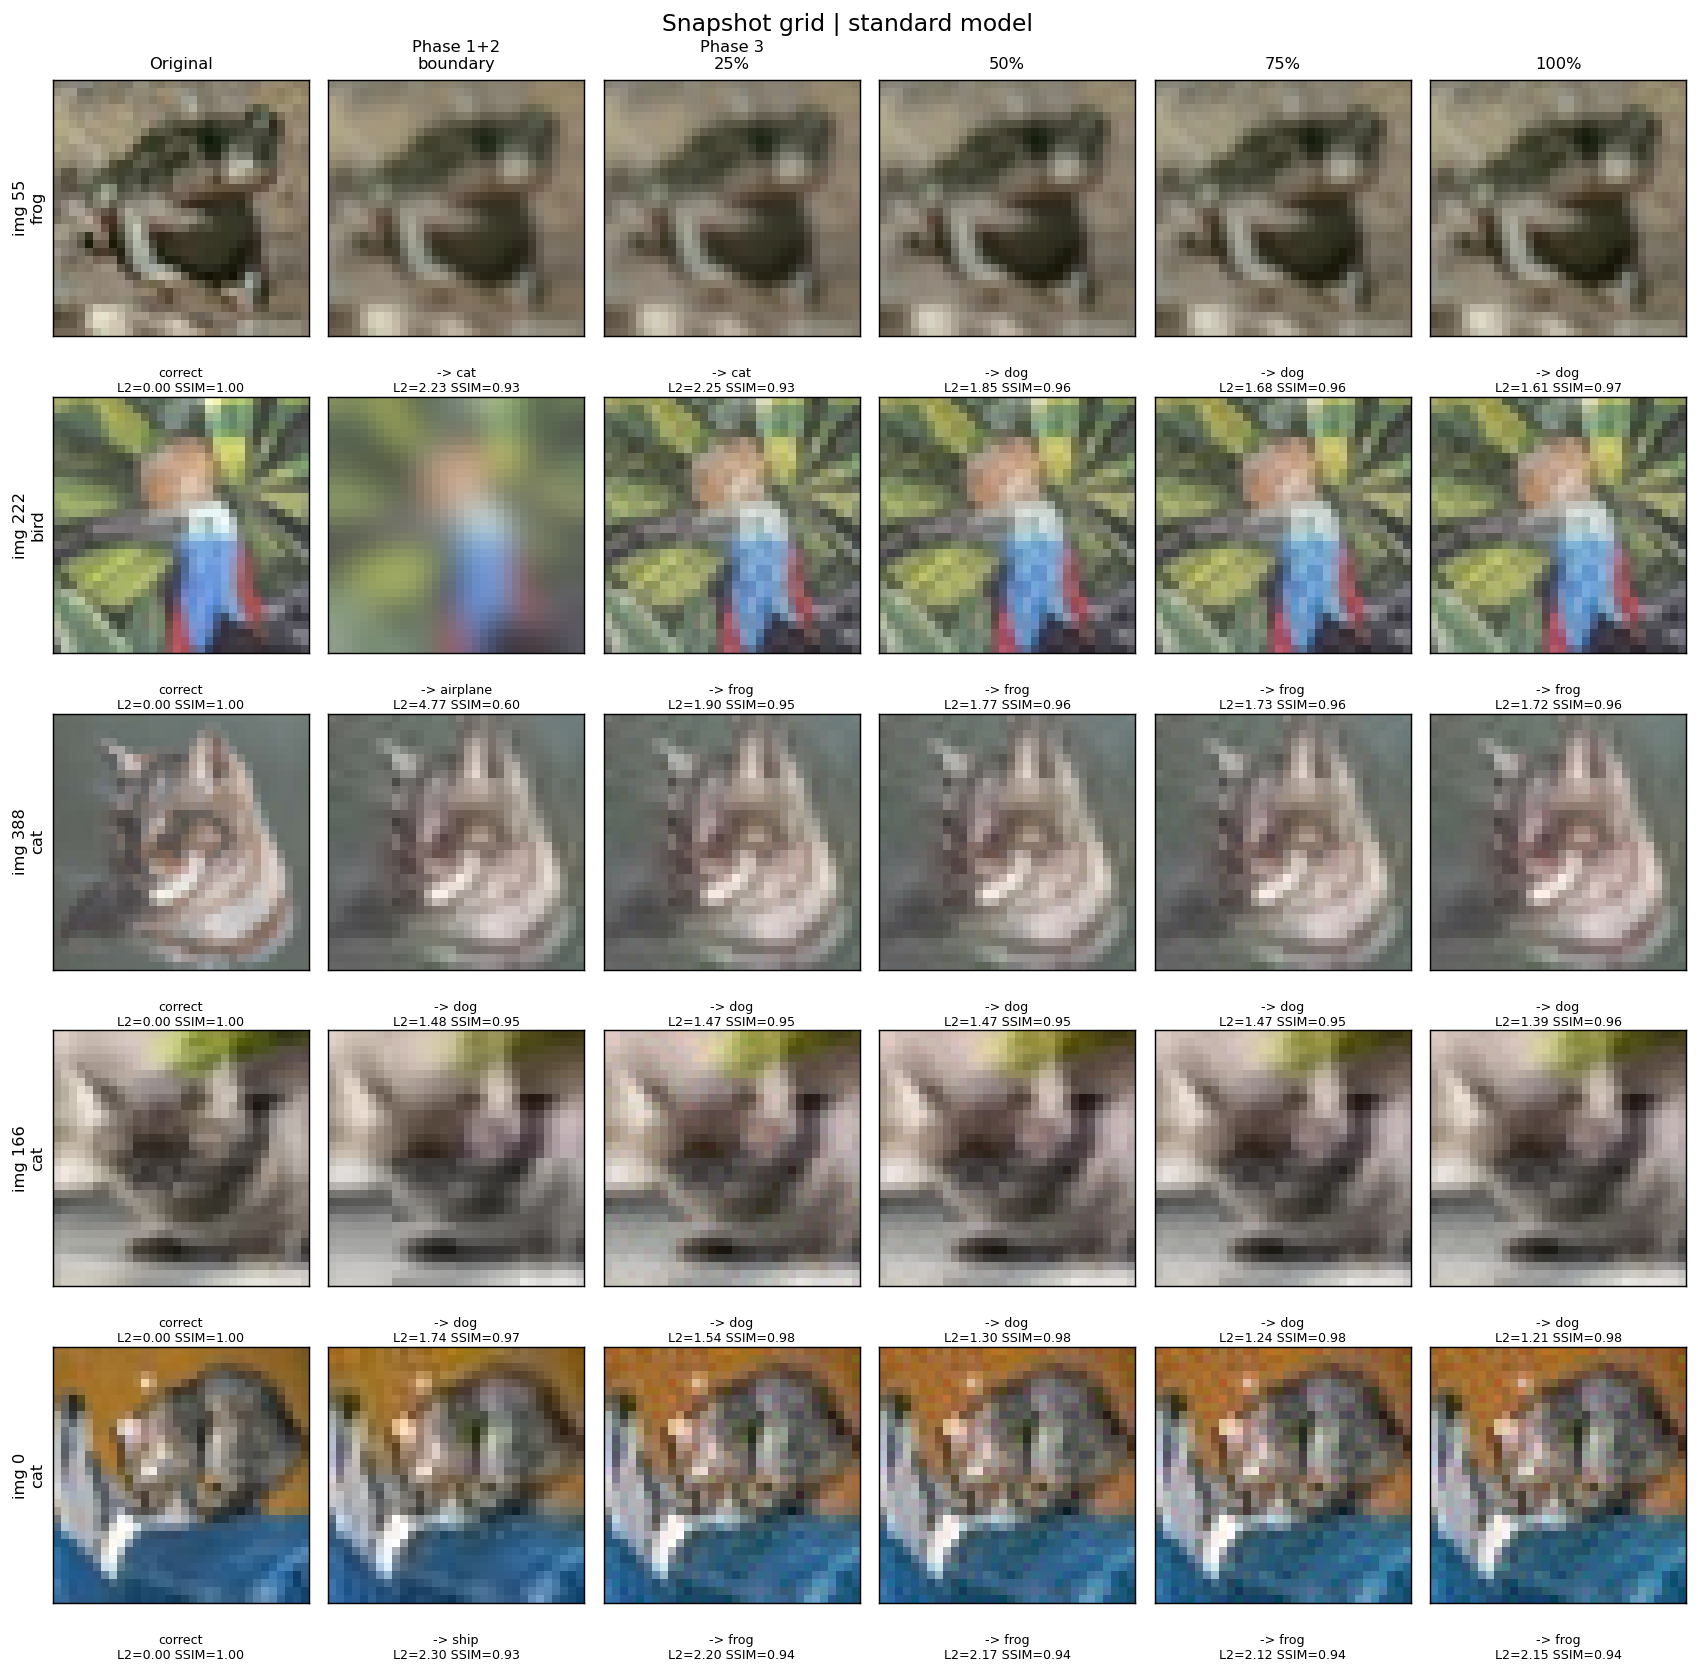
\includegraphics[width=\textwidth]{figures/final_run_snapshot_grid_standard.png}
\caption{Five images tracked through all 6 checkpoints, standard model. Each cell reports the predicted class transition, L2, and SSIM to the original. Phase 1+2 already lands close to the original in most rows; Phase 3 mainly tightens the perturbation further.}
\label{fig:final_grid_standard}
\end{figure}

\begin{figure}[htbp]
\centering
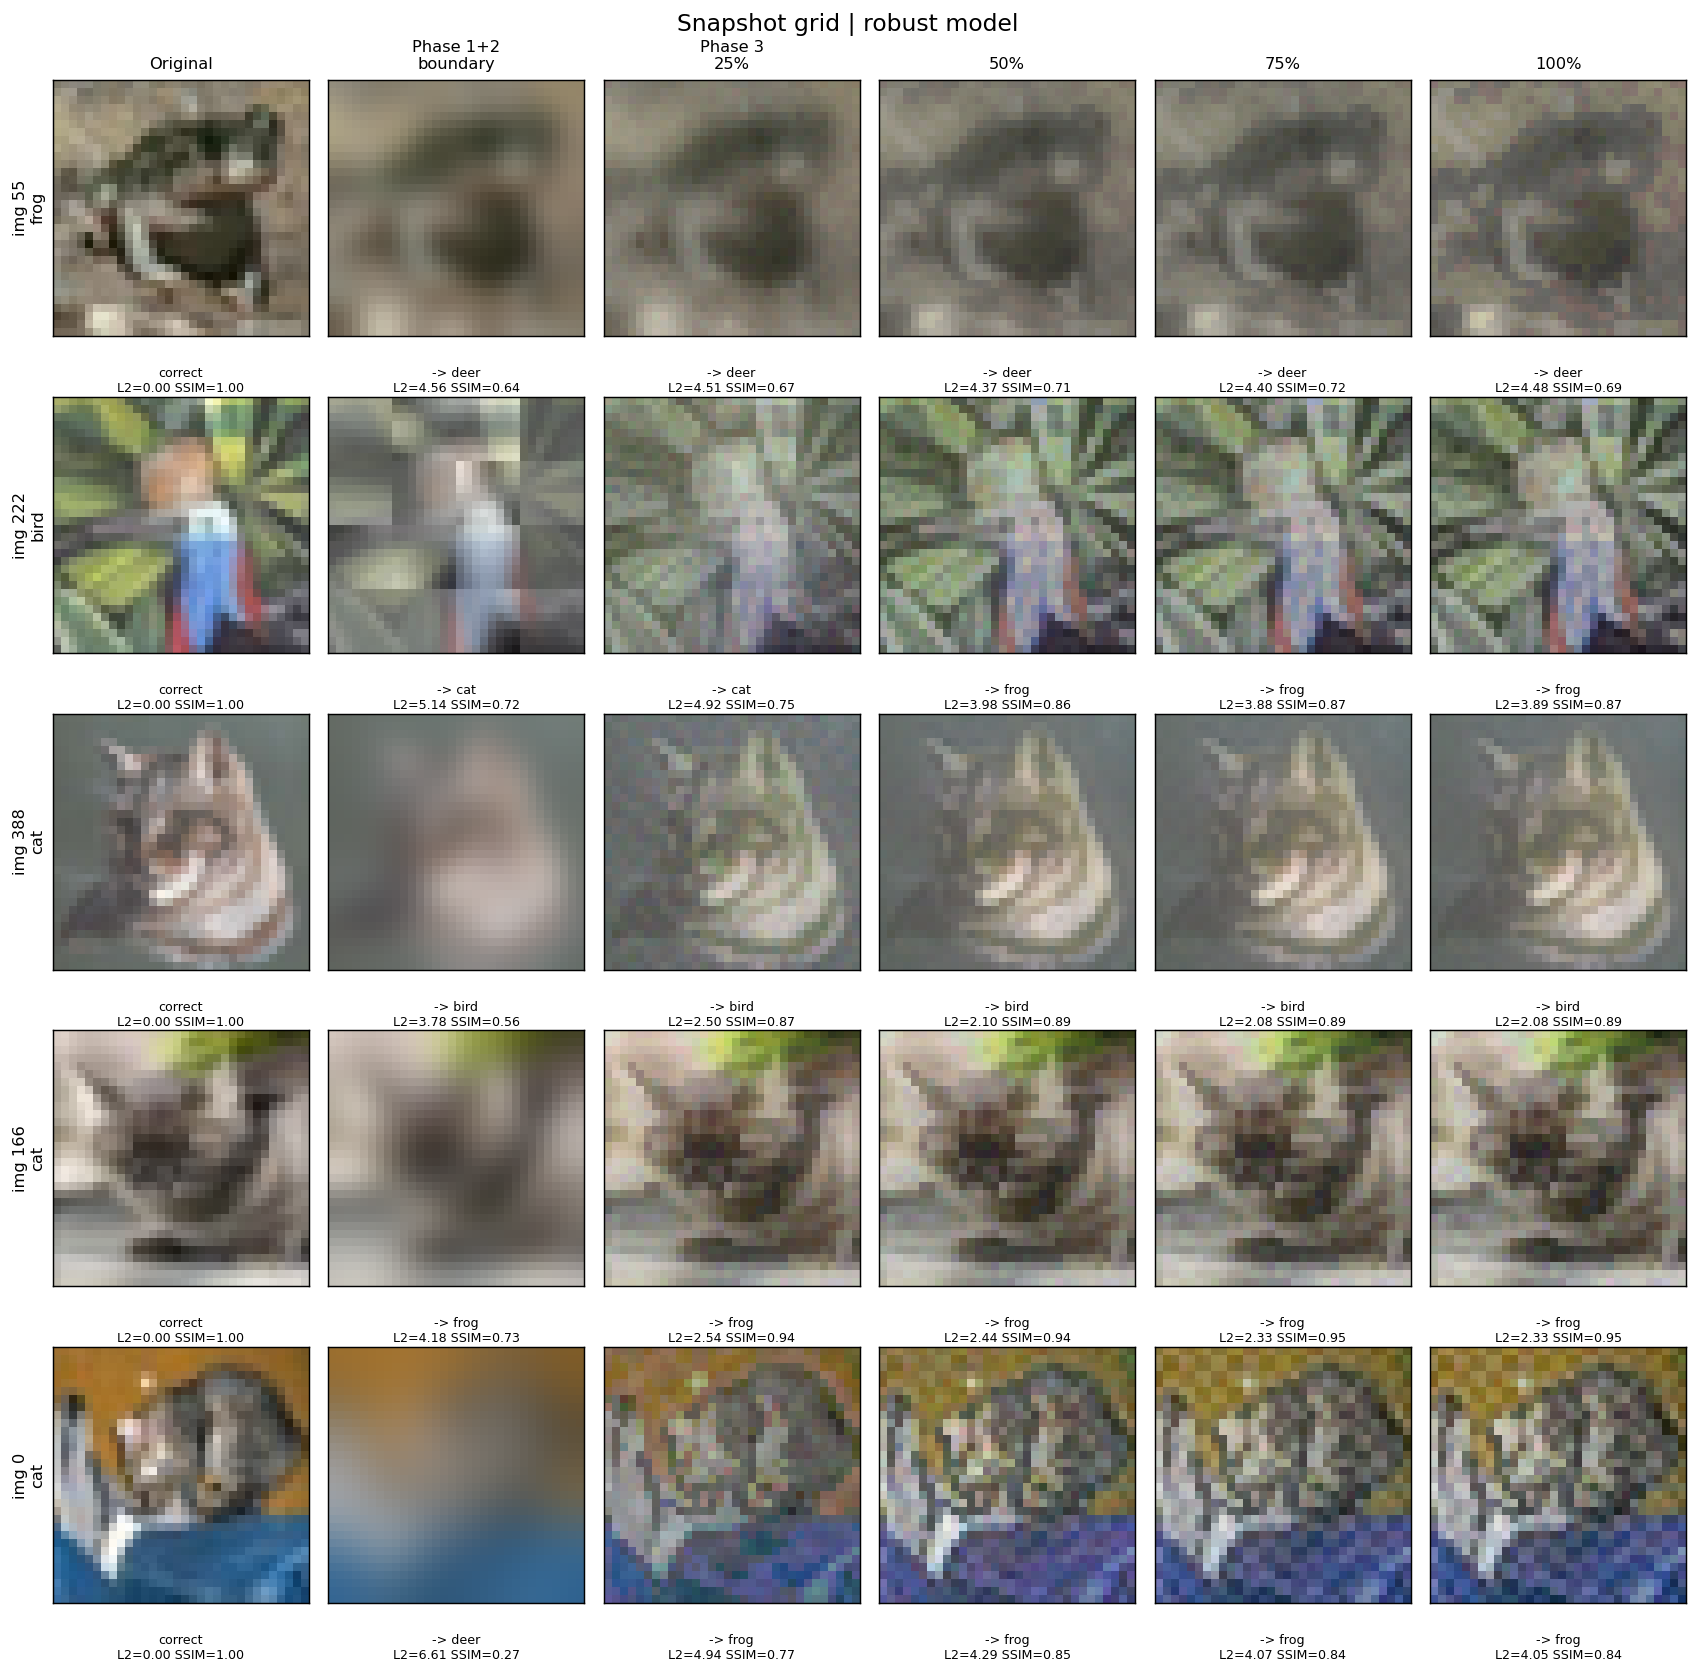
\includegraphics[width=\textwidth]{figures/final_run_snapshot_grid_robust.png}
\caption{Same five images and checkpoints, robust model. The Phase 1+2 boundary point is visibly degraded (low SSIM), but Phase 3 visibly restores structure and SSIM by the 100\% checkpoint in every row, the qualitative counterpart to the IR$_\text{phase3}$ gain in Table~\ref{tab:final_run}.}
\label{fig:final_grid_robust}
\end{figure}

\textbf{Phase 3 is doing real, visible cleanup work, especially against the robust model.} Comparing the ``Phase 1+2 boundary'' and ``100\%'' columns above, the robust-model rows show a clear visual recovery of structure and SSIM across the Phase 3 trajectory, whereas several standard-model rows show comparatively little change because Phase 1+2 already left almost nothing for Phase 3 to fix. This is not specific to the five images plotted: the IR$_\text{phase3}$ distribution is broad and centred well above zero on \emph{both} models (mean $0.223$ standard, $0.219$ robust), and the resulting best-L2 distributions are tight and well-separated by model, with no heavy tail of catastrophic failures at this larger $N$.

\textbf{Good results need far less than the full query budget.} Figure~\ref{fig:final_run_l2q} plots mean L2 against cumulative queries (Phase 1 + Phase 3) for both models. The curve is steep early and flattens well before $Q=2000$ is exhausted: by query $500$ (a quarter of the budget), the mean L2 has already captured $46\%$ (standard) / $50\%$ (robust) of its \emph{total} improvement over the run; by query $1{,}000$ (half the budget), this rises to $78\%$ / $85\%$. In practice this means a usable result is achievable in as few as $500$ queries, five-to-six times smaller than the original paper's $30{,}000$-query regime on ImageNet, consistent with the much lower-dimensional CIFAR-10 setting this report targets throughout. Even so, the curve does not reach zero: both models' Phase 3 keeps tapering off rather than truly converging, the same plateau diagnosed in Part 1, now at a far more favourable level.

\begin{figure}[htbp]
\centering
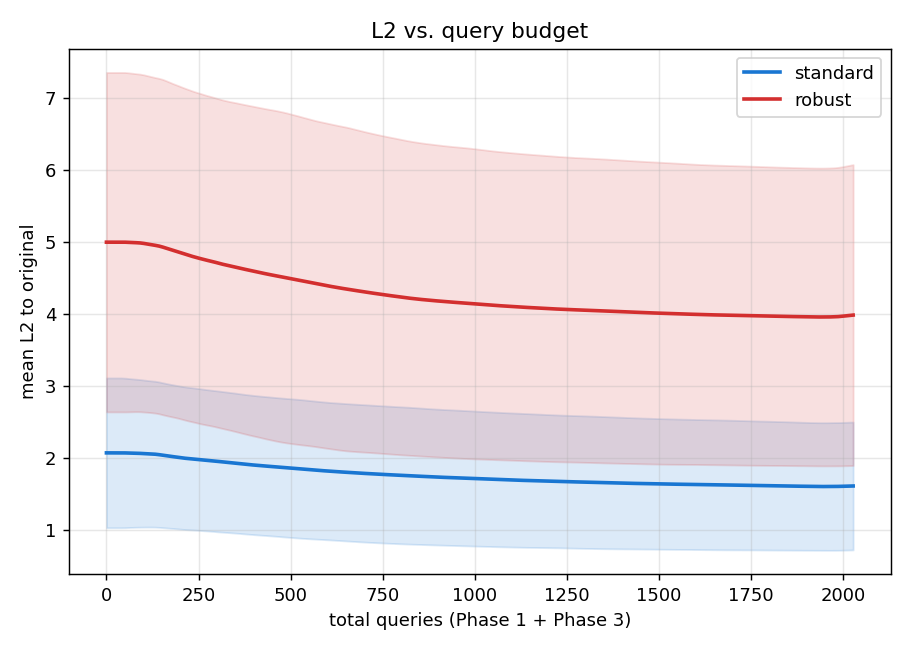
\includegraphics[width=0.8\textwidth]{figures/final_run_l2_vs_query.png}
\caption{Mean L2 vs.\ cumulative queries (Phase 1 + Phase 3), $\pm 1$ std.\ band, both models. Both curves are front-loaded: roughly half of the total improvement is captured by query $500$--$1{,}000$, well short of the $Q=2000$ budget.}
\label{fig:final_run_l2q}
\end{figure}

% =============================================================================
\section{Discussion}
% =============================================================================

\subsection{Where the Improvement Comes From}

Ranking the three contributors established above by impact: \textbf{corruption Phase 1} is by far the largest (Q1, \S\ref{sec:q1_phase1}); initialisation alone, with no change to Phase 3 at all, already accounts for most of the total gain. \textbf{The structured corruption subspace} is the second-largest factor and the one most responsible for breaking the robust model's plateau specifically: Q2's random-subspace control showed that dimensionality reduction alone buys almost nothing, so it is the corruption directions' structure, not merely their number, that lets Phase 3 make progress. \textbf{Population size within the subspace} (Q3) is a real but modest refinement on top of both, with clearly diminishing returns past $\lambda/k\approx2$.

% =============================================================================
\section{Limitations}
\label{sec:limitations}
% =============================================================================

This project is best read as a proof of concept that surfaced a small number of clear, actionable insights (the value of corruption-based initialisation, the case for a subspace search, the limits of pixel-space tuning) rather than as a fully validated benchmark study. Within the time and compute budget available, we prioritised breadth across the investigation, diagnosis, two pixel-space attempts, and the subspace redesign, over exhaustively re-validating every choice at every stage. The gaps below follow from that tradeoff, and are flagged so a reader can judge how far the headline numbers should be trusted, not as an indictment of the result: the core findings (corruption Phase 1's dominance, the subspace's structure mattering more than its size, pixel-space's dimensionality ceiling) are each supported by a dedicated controlled comparison and are, we think, on solid footing.

\subsection{Methodology}

Every comparison in this report is a single point estimate (a mean, a median, or a win rate) rather than a statistical test: we do not run multiple random seeds per image, and we do not report confidence intervals or p-values anywhere. Doing so properly, repeating every condition across several seeds and computing significance, would have multiplied the compute and wall-clock cost of an already large experimental matrix (Parts 1 and 2 together cover well over a dozen distinct conditions across two models), which the project's budget did not allow. The same constraint shaped the overall scope: every result here is specific to CIFAR-10, two WideResNet-28-10 checkpoints (one undefended, one TRADES-trained), and the L2 norm, with no attempt to validate the same findings on other datasets, architectures, defenses, or threat models. The same $N{\approx}200$ image sample is also typically used both to choose a configuration and to report its final numbers, with no separate held-out test split, so the absolute numbers should be read as indicative rather than as a tightly externally-validated estimate. None of this is specific to any one part of the pipeline; it is a property of the project's scope as a whole.

\subsection{Open Questions for Future Work}

\textbf{Hyperparameter choices were not re-validated at every stage.} Attempt 1's tuning conclusions (\S\ref{sec:finetuning}) do not all transfer cleanly to other population sizes, and later experiments, Attempt 2's covariance comparison and all of Part 2's subspace work, continued to use some of the paper's untuned defaults rather than re-tuning every hyperparameter for the new setting each time. A more thorough study would revisit every hyperparameter at every stage rather than carrying earlier defaults forward.

\textbf{\texttt{DIRECTION\_ZOO}'s severities are undocumented constants.} The 8 fixed-parameter corruption functions in the subspace basis (Table~\ref{tab:direction_zoo}) use hardcoded severities that were chosen arbitrarily, with no specific justification beyond the fact that they work. We argue this matters less for a search-space basis than it would for Phase 1 (\S\ref{sec:subspace_construction}), but it remains an unprincipled choice that was never swept or ablated.

\textbf{Several natural extensions remain open.} We never investigated why some images are far easier or harder to corrupt than others, despite a large per-image spread underlying every mean and median in this report; never swept the subspace dimensionality $k$ itself; and never let the basis adapt mid-run rather than freezing it before Phase 3 starts. We also never built a jump-operator analogue using the new corruption subspace (the original jump operator was simply dropped, \S\ref{sec:our_impl}, with nothing tried in its place), and never tested other standard mechanisms for escaping ES stagnation, such as IPOP restarts or an island model running several parallel attacks on the same image. Any of these would be a reasonable next step, time and resources permitting.

% =============================================================================
\section{Conclusion}
% =============================================================================

We implemented and studied EvolBA~\cite{evolba2024} on CIFAR-10 with two WideResNet-28-10 target models (standard and TRADES-robust), progressing through two parts of increasing sophistication.

\textbf{Part 1 (Diagnosis and the Limits of Pixel-Space Fixes)} instrumented the baseline end-to-end and found that most of the query budget is spent on the directed step and its backtracking rather than genuine search, and that Phase 3 plateaus almost immediately against the robust model regardless of where it starts. (A third diagnostic finding, a cheap, effective alternative to fractal initialisation, is described in Part 2 below, where it is actually put to use.) Two attempts to fix this entirely within pixel space, hyperparameter tuning and richer covariance structure, both failed to move the needle by any meaningful amount. Together they point to the same conclusion: the plateau is a problem of search-space dimensionality, not of hyperparameters or covariance representation.

\textbf{Part 2 (Inductive Bias in the Search Space)} addressed that dimensionality problem directly by searching in a small subspace built from corruption directions instead of raw pixels. This substantially raised the ceiling that Part 1's attempts could not lift, an improvement that is most pronounced against the robust model, where pixel-space search had made almost no progress at all, though it does not eliminate the underlying plateau entirely (\S\ref{sec:final_run}).

The overall lesson is that the largest gains in this setting came not from tuning the evolutionary strategy itself, but from reshaping the space it searches in using cheap, problem-specific structure discovered during diagnosis.

\begin{thebibliography}{9}

\bibitem{evolba2024}
A.\ Tajima and S.\ Ono.
\newblock EvolBA: Evolutionary Boundary Attack under Hard-label Black Box condition.
\newblock \textit{arXiv:2407.02248v3}, 2024.

\bibitem{ba2017}
W.\ Brendel, J.\ Rauber, and M.\ Bethge.
\newblock Decision-based adversarial attacks: Reliable attacks against black-box machine learning models.
\newblock \textit{arXiv:1712.04248}, 2017.

\bibitem{wang2023}
Z.\ Wang et al.
\newblock Better diffusion models further improve adversarial training.
\newblock \textit{ICML}, 2023.

\end{thebibliography}

\appendix
\section{Experimental Parameters}

\begin{table}[htbp]
\centering
\caption{Fixed parameters across all experiments.}
\begin{tabular}{ll}
\toprule
Parameter & Value \\
\midrule
Dataset & CIFAR-10, $32 \times 32$ RGB ($n = 3072$) \\
Standard model & WRN-28-10, CE training ($\sim$93\% clean acc.) \\
Robust model   & WRN-28-10, Wang2023 / TRADES ($\sim$92.4\% clean, $\sim$67.3\% robust) \\
Image sample   & 100--200 images jointly correct on both models \\
\midrule
\multicolumn{2}{l}{\textit{Part 1 pixel-space settings:}} \\
Query budget $Q$ & 2{,}000 \\
Default $\lambda$ & $4 + \lfloor 3\ln n \rfloor = 28$ \\
Phase 2 binary search & 26 steps or adaptive (\texttt{bs\_adaptive}) \\
Best validated config & $\xi_{\text{step\_scale}}=0.5$, $\tau=0$, $\lambda=14$, \texttt{bs\_adaptive=True} \\
\midrule
\multicolumn{2}{l}{\textit{Part 2 subspace settings:}} \\
Query budget $Q$ & 1{,}500 \\
Subspace & 11 DIRECTION\_ZOO + 3 DCT bands, QR-orthogonalised, $k\leq14$ \\
Fixed Phase 1 & jpeg + blur + fractal\_random binary search ($\approx141$ queries) \\
Sep-CMA-ES & diagonal $D$, $c_1/c_\mu$ from CMA-ES formulas at dimension $k$ \\
Best validated config & $\lambda=56$, sep-CMA-ES, fixed Phase 1, $k=14$ \\
\bottomrule
\end{tabular}
\end{table}

\section{Code Structure}

All experiments are reproducible from the project repository. Part 1 (pixel-space baseline, hyperparameter tuning, and covariance variants) lives in \texttt{STAGE\_0}/\texttt{STAGE\_1}/\texttt{STAGE\_2}; each study follows the pattern \texttt{run\_studyN.py} (supports \texttt{--mock}) $\to$ \texttt{results.parquet} $\to$ \texttt{make\_studyN\_results.py} $\to$ \texttt{studyN\_results.ipynb}. Part 2's subspace construction and sep-CMA-ES-in-subspace implementation live in \texttt{STAGE\_3}, principally \texttt{attacks/utils/subspace.py} (\texttt{corruption\_basis()}, \texttt{dct\_band\_vector()}) and the Experiment 4/5 population-study scripts in the same directory.

\end{document}
